% !TEX TS-program = lualatex
% =====================================================================
%  TimeLens: On-Device Detection and Retrieval-Grounded Bilingual Q&A for the Grand Egyptian Museum
%  Graduation Project Thesis -- Capital University, FCAI
%  Build:  latexmk main.tex           (XeLaTeX + BibTeX; engine set in .latexmkrc)
%  If IEEEtran.bst is missing, change \bibliographystyle below to plainnat.
% =====================================================================
\documentclass[12pt,a4paper,oneside]{report}

% =====================================================================
%  TimeLens / GEM Graduation Thesis -- shared preamble
%  Compile with pdfLaTeX + BibTeX (latexmk -pdf main.tex).
%  Portable: all packages ship with a full TeX Live / MiKTeX install.
%  NOTE on Arabic: examples are given in transliteration (Latin script)
%  so the document compiles under pdfLaTeX. To typeset native Arabic,
%  switch to XeLaTeX/LuaLaTeX and add fontspec + polyglossia with an
%  Arabic font; no other change is required.
% =====================================================================

% ---- Encoding & fonts -------------------------------------------------
\usepackage[utf8]{inputenc}
\usepackage[T1]{fontenc}
\usepackage{lmodern}
\usepackage{microtype} % char protrusion + font expansion: trims overfull boxes

% ---- Page geometry ----------------------------------------------------
\usepackage[a4paper,left=30mm,right=25mm,top=25mm,bottom=25mm]{geometry}
\usepackage{setspace}
\onehalfspacing

% ---- Math -------------------------------------------------------------
\usepackage{amsmath}
\usepackage{amssymb}

% ---- Graphics & tables ------------------------------------------------
\usepackage{graphicx}
\graphicspath{{figures/}}
\usepackage{booktabs}
\usepackage{array}
\renewcommand{\arraystretch}{1.4} % more vertical breathing room between table rows
\usepackage{multirow}
\usepackage{tabularx}
\usepackage{caption}
\captionsetup{font=small,labelfont=bf}
\usepackage[inline]{enumitem}
\usepackage{longtable}
\usepackage{placeins}

% ---- Colour -----------------------------------------------------------
\usepackage{xcolor}
\definecolor{gemgold}{RGB}{198,153,61}
\definecolor{gemobsidian}{RGB}{20,24,33}
\definecolor{gemblue}{RGB}{31,78,121}
\definecolor{gemgreen}{RGB}{60,120,80}
\definecolor{gemsand}{RGB}{245,240,228}

% ---- Diagrams ---------------------------------------------------------
\usepackage{tikz}
\usetikzlibrary{positioning,arrows.meta,shapes.geometric,fit,backgrounds,calc,shadows.blur}
\usepackage{pgfplots}
\pgfplotsset{compat=1.17}

% reusable node styles for the architecture diagrams
\tikzset{
  block/.style   ={rectangle,rounded corners=3pt,draw=gemblue!70,fill=gemblue!10,
                   align=center,minimum height=10mm,minimum width=26mm,font=\small},
  store/.style   ={rectangle,rounded corners=3pt,draw=gemgreen!70,fill=gemgreen!12,
                   align=center,minimum height=10mm,minimum width=26mm,font=\small},
  edgenode/.style={rectangle,rounded corners=3pt,draw=gemgold!80,fill=gemgold!15,
                   align=center,minimum height=10mm,minimum width=26mm,font=\small},
  flow/.style    ={-{Stealth[length=2.4mm]},thick,draw=gemobsidian!70},
}

% ---- Algorithms -------------------------------------------------------
\usepackage[ruled,vlined,linesnumbered]{algorithm2e}

% ---- Callout / "insight" boxes ---------------------------------------
\usepackage[most]{tcolorbox}
\newtcolorbox{insightbox}[1][Core Insight]{%
  enhanced,breakable,colback=gemblue!5,colframe=gemblue!70!black,
  coltitle=white,fonttitle=\bfseries,title={#1},
  boxrule=0.8pt,arc=2pt,left=3mm,right=3mm,top=2mm,bottom=2mm}

% ---- Bibliography (numeric, IEEE-style) -------------------------------
% natbib + IEEEtran gives "[1]"-style numbering. If IEEEtran.bst is not
% available on your TeX install, change the style in main.tex to plainnat.
\usepackage[numbers,sort&compress]{natbib}

% ---- Hyperlinks (load last) ------------------------------------------
\usepackage{hyperref}
\hypersetup{
  colorlinks=true,
  linkcolor=gemblue!60!black,
  citecolor=gemgreen!55!black,
  urlcolor=gemblue!70!black,
  pdftitle={TimeLens: AI and AR Museum Guide for Egyptian Artifact Recognition},
  pdfauthor={Ali Ashraf, Amr Ahmed, Malak Alaa, Omar Ahmed, Omar Wagih, Rawan Hesham}
}

% ---- Small helpers ----------------------------------------------------
\newcommand{\TimeLens}{\textsc{TimeLens}}
\newcommand{\GEM}{Grand Egyptian Museum}
% en-dash for numeric ranges in text
\newcommand{\range}[2]{#1\,--\,#2}


\begin{document}

% ---------------------------------------------------------------- front
\pagenumbering{roman}             % title page = "i" (hidden); avoids a duplicate
\begin{titlepage}
\thispagestyle{empty}
\centering

\begin{center}

\includegraphics[width=0.25\linewidth]{logo.png}
\end{center}

{\large Capital University\par}
{\large Faculty of Computers and Artificial Intelligence\par}

\vfill

{\LARGE\bfseries TimeLens:\\
	On-Device Artifact Detection and\\
	Retrieval-Grounded Bilingual Q\&A\\
	for the Grand Egyptian Museum\par}

\vspace{8mm}
{\large\itshape A Graduation Project Submitted in the partial fulfillment of B.S. degree in Computer Science \& Artificial Intelligence.\par}

\vfill

\begin{tabular}{@{}ll@{}}
\textbf{Author(s):}      & Ali Ashraf,\; Amr Ahmed,\; Malak Alaa,\\
                         & Omar Ahmed,\; Omar Wagih,\; Rawan Hesham\\[2mm]
\textbf{Supervisor:}     & Dr.\ Islam Gamal\\[2mm]
%\textbf{Degree Sought:}  & B.Sc.\ in Artificial Intelligence\\[2mm]
\textbf{Submission Date:}& June 2026\\
\end{tabular}

\vfill

\end{titlepage}
     % arabic "page.1" anchor colliding with Chapter 1
\setcounter{page}{2}              % front matter proper then continues at "ii"

\chapter*{Declaration of Originality}
\addcontentsline{toc}{chapter}{Declaration of Originality}

We declare that this thesis and all included chapters represent our original
academic work, except where properly cited. All external datasets, open-source
libraries, prior papers, and AI-assisted outputs are disclosed and attributed.
The intellectual core, experimental design, implementation decisions, and
critical evaluation were performed by the student team.

\vspace{2cm}
\noindent
\begin{tabular}{@{}p{0.5\textwidth}p{0.4\textwidth}@{}}
Signature(s): \hrulefill & Date: \hrulefill \\
\end{tabular}

\chapter*{Abstract}
\addcontentsline{toc}{chapter}{Abstract}

This thesis documents the design, implementation, and evaluation of \TimeLens{},
an AI- and AR-powered mobile guide for the \GEM{} (GEM). Pointing a phone at an
exhibit, a visitor sees the artifact recognized in real time and can ask follow-up
questions answered in English or Arabic. The work targets three problems specific
to in-gallery deployment: fine-grained visual similarity among \textbf{51 catalogued
artifacts} (many near-identical Ramesside statues), the gap between curated training
data and handheld phone-camera conditions, and the risk of an AI guide stating
historical ``facts'' it cannot support.

The thesis presents two engineering-research contributions and a market study. The
first is an \textbf{on-device artifact detector} developed through a
data-quality-driven iteration study: from foundation-model auto-annotation
(YOLO-World), through spatial label-cleaning rules, to a fully hand-annotated
dataset. The study isolates \emph{label quality}---rather than model architecture or
input resolution---as the decisive factor: the final \textbf{YOLOv8n} model resolves
every previously failing class while remaining a \textbf{5.97\,MB} TensorFlow Lite
asset that runs in real time on a mid-range phone. The second is a \textbf{bilingual
Retrieval-Augmented Generation (RAG) guide} grounded in a \textbf{108-record ChromaDB}
knowledge base; a systematic benchmark of \textbf{seven candidate language models}
selects \textbf{Gemma 4 E2B (Q4\_K\_M)}, and a ten-step optimization reduces
end-to-end latency from \textbf{over 30\,s to about 10\,s}. Both ship in a production
\textbf{Flutter} application with a bilingual interface, museum location gating, and
text-to-speech.

Beyond headline metrics, the thesis is written to be reproducible and honest about
its limits: the detection study explicitly discloses validation \emph{frame-leakage}
and the training-to-deployment \emph{domain shift}, reporting a conservative held-out
result (mAP@0.5 $=0.751$) alongside the in-distribution figures. The document
includes reproducibility notes, an ethics and bias statement, and a formal
generative-AI disclosure.

\begin{insightbox}
A reliable museum guide is built less by adding model complexity than by
\emph{grounding} it: clean labels make the on-device detector trustworthy, and
retrieval-grounded generation keeps the language model factual. \TimeLens{}'s value
comes from disciplined data and grounding, not a larger model.
\end{insightbox}

\chapter*{Graphical Abstract}
\addcontentsline{toc}{chapter}{Graphical Abstract}

\vspace*{0.5em}
\begin{center}
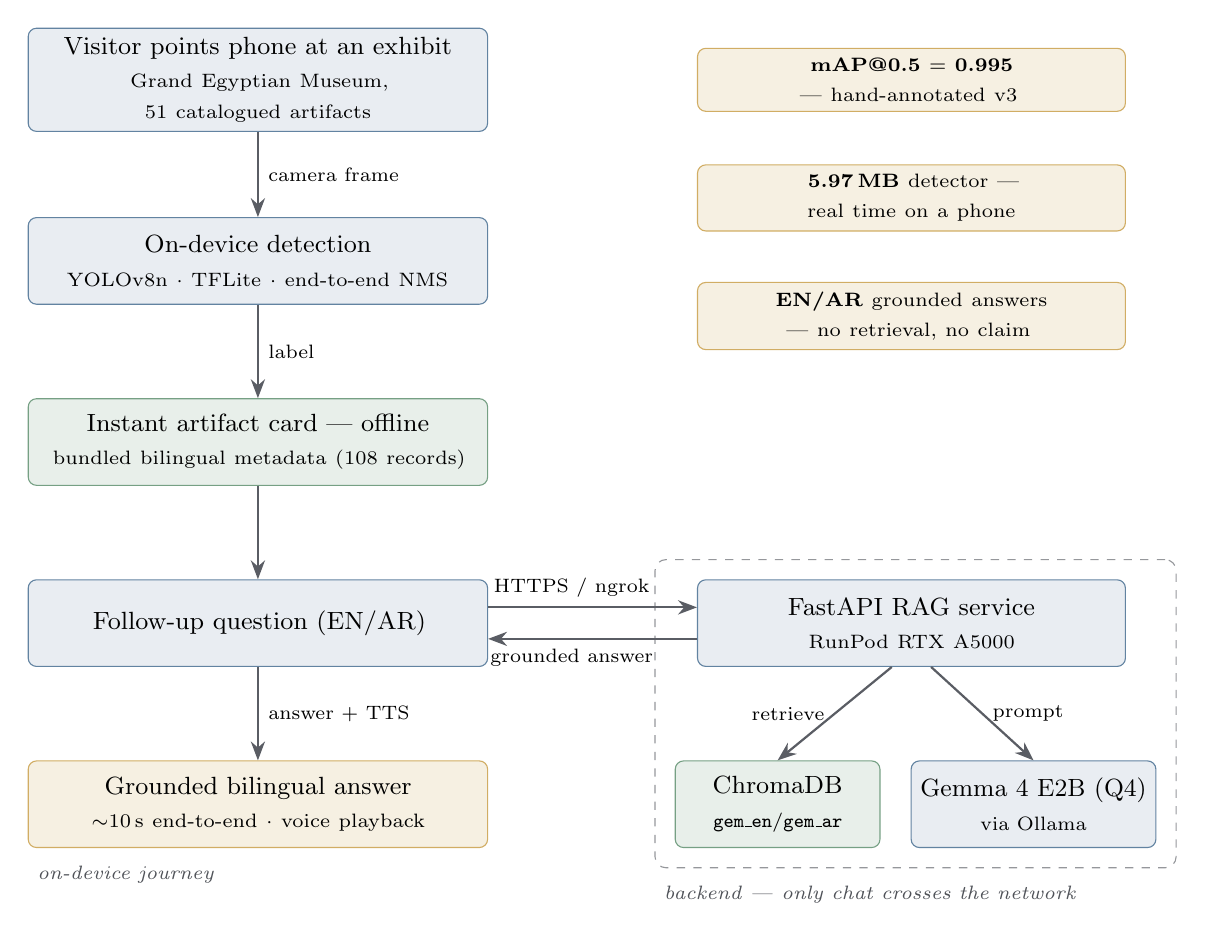
\begin{tikzpicture}[every node/.style={font=\small}]
  % ---- visitor journey (left lane) -----------------------------------
  \node[block,text width=56mm,minimum height=11mm] (n1) at (0,0)
    {Visitor points phone at an exhibit\\[1pt]\scriptsize Grand Egyptian Museum, 51 catalogued artifacts};
  \node[block,text width=56mm,minimum height=11mm] (n2) at (0,-2.3)
    {On-device detection\\[1pt]\scriptsize YOLOv8n $\cdot$ TFLite $\cdot$ end-to-end NMS};
  \node[store,text width=56mm,minimum height=11mm] (n3) at (0,-4.6)
    {Instant artifact card --- offline\\[1pt]\scriptsize bundled bilingual metadata (108 records)};
  \node[block,text width=56mm,minimum height=11mm] (n4) at (0,-6.9)
    {Follow-up question (EN/AR)};
  \node[edgenode,text width=56mm,minimum height=11mm] (n5) at (0,-9.2)
    {Grounded bilingual answer\\[1pt]\scriptsize $\sim$10\,s end-to-end $\cdot$ voice playback};
  \draw[flow] (n1) -- node[right,font=\scriptsize]{camera frame} (n2);
  \draw[flow] (n2) -- node[right,font=\scriptsize]{label} (n3);
  \draw[flow] (n3) -- (n4);
  \draw[flow] (n4) -- node[right,font=\scriptsize]{answer $+$ TTS} (n5);

  % ---- key results (right, top) --------------------------------------
  \node[edgenode,text width=52mm,minimum height=8mm] (k1) at (8.3,0)
    {\scriptsize\textbf{mAP@0.5 $=$ 0.995} --- hand-annotated v3};
  \node[edgenode,text width=52mm,minimum height=8mm] (k2) at (8.3,-1.5)
    {\scriptsize\textbf{5.97\,MB} detector --- real time on a phone};
  \node[edgenode,text width=52mm,minimum height=8mm] (k4) at (8.3,-3.0)
    {\scriptsize\textbf{EN/AR} grounded answers --- no retrieval, no claim};

  % ---- backend (right, bottom) ----------------------------------------
  \node[block,text width=52mm,minimum height=11mm] (b1) at (8.3,-6.9)
    {FastAPI RAG service\\[1pt]\scriptsize RunPod RTX A5000};
  \node[store,text width=21mm,minimum height=11mm] (b2) at (6.6,-9.2)
    {ChromaDB\\[1pt]\scriptsize \texttt{gem\_en}/\texttt{gem\_ar}};
  \node[block,minimum height=11mm,align=center] (b3) at (9.85,-9.2)
    {Gemma 4 E2B (Q4)\\[1pt]\scriptsize via Ollama};
  \begin{scope}[on background layer]
    \node[draw=gemobsidian!45,dashed,rounded corners=4pt,inner sep=2.5mm,
          fit=(b1)(b2)(b3)] (bk) {};
  \end{scope}
  \draw[flow] ([yshift=2mm]n4.east) -- node[above,font=\scriptsize,pos=0.4]{HTTPS / ngrok} ([yshift=2mm]b1.west);
  \draw[flow] ([yshift=-2mm]b1.west) -- node[below,font=\scriptsize,pos=0.6]{grounded answer} ([yshift=-2mm]n4.east);
  \draw[flow] ($(b1.south)+(-2.5mm,0)$) -- node[left,font=\scriptsize]{retrieve} (b2.north);
  \draw[flow] ($(b1.south)+(2.5mm,0)$) -- node[right,font=\scriptsize]{prompt} (b3.north);

  % ---- lane tags -------------------------------------------------------
  \node[font=\scriptsize\itshape,text=gemobsidian!75,anchor=north west]
    at ([yshift=-1mm]n5.south west) {on-device journey};
  \node[font=\scriptsize\itshape,text=gemobsidian!75,anchor=north west]
    at ([yshift=-1mm]bk.south west) {backend --- only chat crosses the network};
\end{tikzpicture}
\end{center}

\vspace{0.8em}
\noindent\textsc{TimeLens} in one view: artifact identity is decided entirely on the
phone by a hand-annotation-driven YOLOv8n detector and answered instantly from
bundled bilingual metadata; only a follow-up chat question crosses the network, where
a FastAPI service grounds Gemma in ChromaDB retrieval so every claim traces back to
curated museum data.

\chapter*{Acknowledgment}
\addcontentsline{toc}{chapter}{Acknowledgment}

We thank our supervisor, Dr.\ Islam Gamal, and the faculty mentors and peers at the
Faculty of Computers and Artificial Intelligence, Helwan University, for their
continuous guidance. We are also grateful to the open-source community whose tools
---Ultralytics, Flutter, Ollama, ChromaDB, LlamaIndex, and many others---made rapid
experimentation and deployment possible.

\chapter*{Dedication}
\addcontentsline{toc}{chapter}{Dedication}

Dedicated to everyone working to preserve cultural heritage through responsible
technology.


\tableofcontents
\listoffigures
\listoftables
\listofalgorithms
\chapter*{List of Equations}
\addcontentsline{toc}{chapter}{List of Equations}

\begin{center}
\begin{tabular}{@{}ll@{}}
\toprule
\textbf{Equation Ref.} & \textbf{Description}\\
\midrule
Eq.\ (5.1) & Intersection over Union (IoU)\\
Eq.\ (5.2) & Precision\\
Eq.\ (5.3) & Recall\\
Eq.\ (5.4) & Average Precision (AP)\\
Eq.\ (5.5) & mean Average Precision (mAP@0.5 and mAP@0.5:0.95)\\
\bottomrule
\end{tabular}
\end{center}

\chapter*{List of Abbreviations and Acronyms}
\addcontentsline{toc}{chapter}{List of Abbreviations and Acronyms}

\begin{center}
\begin{tabular}{@{}ll@{}}
\toprule
\textbf{Abbr.} & \textbf{Full Name}\\
\midrule
AI     & Artificial Intelligence\\
AR     & Augmented Reality\\
CNN    & Convolutional Neural Network\\
YOLO   & You Only Look Once\\
NMS    & Non-Maximum Suppression\\
TFLite & TensorFlow Lite\\
mAP    & mean Average Precision\\
IoU    & Intersection over Union\\
FPS    & Frames Per Second\\
RAG    & Retrieval-Augmented Generation\\
LLM    & Large Language Model\\
API    & Application Programming Interface\\
GEM    & Grand Egyptian Museum\\
TTS    & Text-to-Speech\\
RTL    & Right-to-Left (text layout)\\
VRAM   & Video Random-Access Memory\\
\bottomrule
\end{tabular}
\end{center}

\chapter*{Glossary}
\addcontentsline{toc}{chapter}{Glossary}

\begin{center}
\begin{tabular}{@{}p{0.32\textwidth}p{0.6\textwidth}@{}}
\toprule
\textbf{Term} & \textbf{Definition}\\
\midrule
Fine-grained recognition & Classification where classes differ by subtle local details.\\
Auto-annotation & Generating training labels automatically with a foundation model (here, YOLO-World) instead of by hand.\\
Frame leakage & Inflated metrics caused by near-duplicate video frames split across train and validation sets.\\
Domain shift & Performance gap between curated training data and real deployment conditions.\\
End-to-end NMS & A detector export that performs non-maximum suppression inside the model graph.\\
Retrieval-Augmented Generation (RAG) & Grounding a language model's answer in passages retrieved from a knowledge base.\\
Grounding & Constraining generated text to retrieved, verified context to prevent fabrication.\\
Confidence gate & The per-class threshold that admits a detection (unlocking artifact information and chat) or suppresses it so the app keeps scanning.\\
\bottomrule
\end{tabular}
\end{center}

\chapter*{List of Publications}
\addcontentsline{toc}{chapter}{List of Publications}

\begin{enumerate}[leftmargin=2em]
  \item A.\ Ashraf, A.\ Ahmed, M.\ Alaa, O.\ Ahmed, O.\ Wagih, and R.\ Hesham,
        ``AR and AI in Museum Tourism: A Market Analysis of Intelligent Guide
        Systems for Egyptian Cultural Heritage,'' Faculty of Computers and
        Artificial Intelligence, Helwan University, 2026.
\end{enumerate}


% ---------------------------------------------------------------- main
\cleardoublepage
\pagenumbering{arabic}

\chapter{Introduction}

\section{Problem Statement}

Fine-grained artifact recognition in museum environments is difficult due to
background clutter, low-light capture, visual overlap between classes, and open-set
uncertainty. At the \GEM{} (GEM) the difficulty is acute: the target set contains
\textbf{51 catalogued artifacts}, many of which are near-identical Ramesside statues
that differ only in subtle pose, headdress, or accompanying standards. Single-model
solutions trained on idealized imagery often produce unstable predictions in field
conditions.

In practical terms, this means the system can appear confident when it should be
cautious, and uncertain when the visitor expects immediate clarity. A tourist
standing in front of two visually similar statues does not care about model
internals; they care about whether the app gives a trustworthy answer quickly, and
in their own language. This mismatch between academic benchmark success and
real-world reliability is the true problem addressed by this thesis.

\section{Motivation and Significance}

\TimeLens{} is motivated by practical museum needs: reliable visitor guidance,
catalogue support, and safe AI--human interaction. The project targets a
production-ready path where on-device recognition is strong enough to drive a
downstream knowledge experience without sending every camera frame to the cloud.

The significance is both technical and cultural. Technically, the work advances a
\emph{label-quality-driven} recipe for fine-grained visual recognition under
difficult conditions, and a \emph{grounded} bilingual question-answering layer that
resists fabrication. Culturally, it contributes to accessible heritage
interpretation by helping visitors understand artifacts in context, in real time,
and in natural language. The thesis treats this dual objective seriously: high model
quality without user trust is insufficient, and polished UX without reliable identity
and grounding is unsafe.

\begin{insightbox}[The TimeLens Vision]
We don't just recognize artifacts; we unlock their stories. By pairing a compact
\textbf{on-device detector} with a \textbf{retrieval-grounded Gemma guide}, we turn
every smartphone into a bilingual curatorial companion.
\end{insightbox}

\section{Research Gaps, Questions, and Objectives}

\subsection{Research Gaps}
\begin{itemize}[leftmargin=1.5em]
  \item Generic detectors trained on web imagery are weak on fine-grained,
        domain-specific artifacts such as near-identical Ramesside statues.
  \item On datasets built from video frames, naïve random train/validation splits
        leak near-duplicate frames across the split and inflate reported accuracy.
  \item Public-facing museum AI guides hallucinate historical facts when generation
        is not grounded in curated data, and frequently handle Arabic poorly.
\end{itemize}

\subsection{Research Questions}
\begin{itemize}[leftmargin=1.5em]
  \item \textbf{RQ1.} Can label-quality iteration (auto-annotation $\rightarrow$
        cleaning $\rightarrow$ hand-annotation) yield a compact on-device detector
        that reliably distinguishes 51 fine-grained Egyptian artifacts?
  \item \textbf{RQ2.} Can a retrieval-grounded, locally-served language model deliver
        factual, bilingual (English/Arabic) museum answers at interactive latency?
  \item \textbf{RQ3.} Can the combined system run on commodity phones and a single
        small GPU, making it suitable for real museum deployment?
\end{itemize}

\subsection{Objectives}
\begin{itemize}[leftmargin=1.5em]
  \item Build and evaluate a compact, leakage-aware on-device artifact detector
        (YOLOv8n) exported to TensorFlow Lite.
  \item Build a grounded bilingual RAG guide (ChromaDB retrieval + Gemma 4 E2B
        generation) served behind a FastAPI interface.
  \item Integrate both in a Flutter application and document the market relevance of
        AR plus deep learning for heritage technology.
\end{itemize}

\section{Proposed Solution Overview}

\TimeLens{} splits cleanly into an on-device perception layer and a grounded
knowledge layer. On the phone, a compact \textbf{YOLOv8n} detector---exported to
TensorFlow Lite with end-to-end non-maximum suppression---runs on the live camera
feed and classifies the framed exhibit as one of 51 catalogued artifacts, drawing a
tracking box in real time. Because the detector was trained on clean, hand-verified
labels, its confidence is well calibrated: real artifacts score high while off-target
scenes fall below a rejection threshold, so the app can \textbf{trust the on-device
label directly} without a per-frame network round-trip. When the visitor taps a
confident detection, the app opens the artifact's information and a conversational
guide; views that fall below the per-class confidence threshold produce no overlay at
all, so the app simply keeps scanning rather than guessing.

The conversational guide is a bilingual Retrieval-Augmented Generation (RAG)
service. Rather than relying on a language model's parametric memory, it retrieves
the most relevant entries from a curated 108-record ChromaDB knowledge base and
passes them to Gemma 4 E2B---served locally through Ollama behind a FastAPI
endpoint---as grounding context. This keeps every answer anchored to verified museum
data in the visitor's language (English or Arabic) and structurally limits invented
historical claims. A backend re-verification of the on-device label is supported by
the architecture but is not required in the deployed path, where the calibrated
detector is the source of truth.

\section{Thesis Organization}

The remainder of the thesis is organized as follows. Chapter~2 reviews related work
in on-device detection, foundation-model auto-annotation, and retrieval-augmented
generation. Chapter~3 presents the analysis and requirements. Chapter~4 describes the
deployed system architecture. Chapter~5 is the on-device detection study (the
data-quality-driven YOLOv8n contribution). Chapter~6 covers the bilingual RAG guide
and its deployment. Chapter~7 is the market analysis of AR and AI guide systems for
Egyptian cultural heritage. Chapter~8 concludes and outlines future work. Appendices
cover ethics, reproducibility, and a generative-AI disclosure.

\chapter{Literature Review}

\section{Domain Background}

Digital heritage systems require high recognition reliability under uncontrolled
acquisition conditions. Museum deployments add constraints including privacy,
latency, multilingual support, and explainable outcomes.

Unlike lab datasets, museum environments introduce dynamic human behavior: people
move in front of displays, lighting varies across halls, glass reflections appear
unexpectedly, and objects are photographed from oblique angles. A model that performs
well in clean, centered-image conditions can fail abruptly in these scenarios. The
literature review is therefore interpreted through deployment realism rather than
isolated benchmark ranking.

\section{State of the Art in Software Solutions}

Existing solutions include cloud classification APIs, AR image-retrieval systems, and
on-device CNN classifiers. Each approach trades off latency, privacy, and robustness.
Marker-based AR remains common in heritage apps but is sensitive to viewing angle and
lighting and scales poorly to large artifact sets, as documented in case studies of
Egyptian cultural-heritage AR~\citep{abdelhady2025enhancing}.

\section{Survey of AI Approaches}

\subsection{On-Device Object Detection}
Single-stage detectors of the YOLO family provide a strong speed/accuracy balance for
mobile deployment, and export cleanly to TensorFlow Lite for on-device inference with
end-to-end non-maximum suppression baked into the graph~\citep{yolov8}. Comparative
studies of museum-exhibit recognition from video-derived datasets report that YOLOv8
reaches very high mean Average Precision while remaining light enough for real-time
mobile use, outperforming heavier backbones such as VGG-16 and ResNet variants on the
speed/accuracy trade-off~\citep{ipalakova2025comparative}. Adaptive CNN approaches
have likewise been used to enrich museum interaction through automatic artifact
recognition~\citep{wen2024enhancing}.

\subsection{Foundation-Model Auto-Annotation}
Manually annotating tens of thousands of frames is prohibitive for a student-led
project, motivating \emph{auto-annotation} with open-vocabulary, text-prompted
detectors such as YOLO-World~\citep{yoloworld}. Such foundation models handle generic
concepts well but degrade on fine-grained, domain-specific objects---precisely the
near-identical statues that dominate the GEM collection---producing systematically
mislocalized or sibling-confused labels. This limitation is the central motivation for
the data-quality study in Chapter~5.

\subsection{Retrieval-Augmented Generation and On-Device LLMs}
Retrieval-Augmented Generation (RAG) grounds a language model's output in passages
retrieved from a knowledge base rather than its parametric memory, reducing
fabrication in knowledge-intensive tasks~\citep{lewis2020rag}. Recent work also brings
context-aware LLM assistants into AR settings~\citep{qorbani2025teaching}. On the
serving side, quantized models run locally through runtimes such as
Ollama~\citep{ollama}, while multilingual sentence embeddings make a single bilingual
(English/Arabic) retrieval index practical. Robustness challenges specific to heritage
capture---low contrast, reduced lighting for pigment preservation, and crowd
occlusion---are active research topics~\citep{liu2025yolov8,dai2024occlusion}.

\section{Identification of Research Gaps}

The review identifies three combined gaps that this thesis addresses: (i) label
quality for fine-grained, domain-specific detection; (ii) honest evaluation of
video-frame datasets, where random splits leak near-duplicate frames; and (iii)
grounded, bilingual generation for public-facing museum guides. Table~\ref{tab:gaps}
maps prior approaches to how \TimeLens{} fills each gap.

\begin{table}[htbp]
\centering
\caption{Synthesis of prior work and gap fit.}
\label{tab:gaps}
\begin{tabularx}{\textwidth}{@{}>{\raggedright\arraybackslash}p{0.24\textwidth}>{\raggedright\arraybackslash}p{0.20\textwidth}>{\raggedright\arraybackslash}p{0.22\textwidth}>{\raggedright\arraybackslash}X@{}}
\toprule
\textbf{Approach} & \textbf{Strength} & \textbf{Limitation} & \textbf{How TimeLens addresses it}\\
\midrule
Cloud classification APIs & Easy integration, strong models & Latency, privacy, connectivity dependence & On-device YOLOv8n detection (no per-frame round-trip)\\
Foundation-model auto-annotation (YOLO-World) & Cheap labels at scale & Fails on fine-grained, domain-specific artifacts & Label-quality iteration: spatial cleaning $+$ hand annotation\\
Random-split evaluation on video frames & Simple to run & Frame leakage inflates metrics & Honest disclosure $+$ conservative held-out; future video-level split\\
Ungrounded LLM guides & Fluent, engaging & Hallucinate facts; weak Arabic & Bilingual RAG grounding (ChromaDB $+$ Gemma 4 E2B)\\
\bottomrule
\end{tabularx}
\end{table}

\chapter{Analysis and Requirements Engineering}

\section{Stakeholder Analysis}

Primary stakeholders include visitors, curators, research engineers, and operations
teams. Each requires a different quality guarantee: usability, reliability,
explainability, and maintainability. Visitors prioritize speed and clarity; curators
emphasize factual integrity and update control; engineers prioritize maintainability
and reproducibility; leadership focuses on adoption and measurable engagement. A
system that optimizes only one of these viewpoints tends to fail in operation; hence
requirements engineering here explicitly balances all four.

\section{Functional Requirements}

\begin{enumerate}[label=\textbf{FR-\arabic*.},leftmargin=3em]
  \item \textbf{Real-time detection.} Detect and track artifacts in the live camera
        feed with bounding-box overlays at interactive frame rates.
  \item \textbf{On-device classification.} Classify a framed artifact as one of the
        51 catalogued GEM artifacts entirely on-device, with no per-frame network call.
  \item \textbf{Confidence gating.} A confident detection opens the artifact's
        information; a view that falls below the per-class confidence threshold is
        suppressed, so the app keeps scanning instead of guessing.
  \item \textbf{Artifact information.} Present name, period/dynasty, material, and
        description, with an original$\rightarrow$restored image toggle where available.
  \item \textbf{Bilingual AI guide.} Answer artifact-specific and general questions in
        the user's language, grounded in curated museum data.
  \item \textbf{Bilingual UI.} Support full English/Arabic switching including
        right-to-left layout, with the chosen language persisted across sessions.
  \item \textbf{Text-to-speech.} Optionally read AI replies aloud in the active language.
  \item \textbf{Photo capture.} Capture and save camera photos to the device gallery.
  \item \textbf{Museum information and location.} Provide a museum-information screen
        (hours, location, ticketing, map) with location gating for on-site versus
        off-site visitors.
\end{enumerate}

\section{Non-Functional Requirements}

\begin{enumerate}[label=\textbf{NFR-\arabic*.},leftmargin=3.4em]
  \item \textbf{Latency:} real-time on-device detection (target $\geq 2.5$\,FPS
        on a mid-tier Android phone) and AI answers within a few seconds.
  \item \textbf{Footprint:} compact TensorFlow Lite model ($\leq 8$\,MB; actual
        5.97\,MB), installable on low-storage devices.
  \item \textbf{Robustness:} tolerate clutter, overlap, oblique angles, and
        fine-grained confusion among near-identical artifacts.
  \item \textbf{Privacy/edge:} perform recognition on-device with no per-frame
        upload; serve the AI backend locally, avoiding any third-party LLM API.
  \item \textbf{Accessibility:} bilingual content plus text-to-speech audio.
  \item \textbf{Maintainability/scalability:} modular, independently replaceable
        services; the knowledge base is updatable without an app release.
\end{enumerate}

\section{Data Requirements}

\subsection{Data Sources and Acquisition}
Training data consists of roughly 30{,}000 frames extracted (at about one frame per
second) from approximately 50 in-gallery videos of GEM artifacts captured during
the museum's opening hours, spanning all 51 classes. This source reflects the real
deployment domain far better than generic web imagery.

\subsection{Volumetric and Diversity Requirements}
The dataset must cover class diversity, view diversity, and clutter diversity, with
balanced per-class representation. Per-class frame counts range from a few hundred to
just under a thousand, which is reasonably balanced for the task.

\subsection{Annotation and Labeling Standards}
Annotation consistency, class-map governance, and \emph{leakage-aware} split policies
are required. Because frames are extracted from continuous video, adjacent frames are
near-duplicates; splits must therefore be performed \emph{chronologically within each
class/video group} rather than by random shuffle, to avoid leaking near-identical
frames across train, validation, and test (see Chapter~5).

\section{App Persona}

To keep design decisions anchored to a concrete user rather than an abstract average,
we model a representative visitor (Figure~\ref{fig:persona}). Her goals and frustrations
motivate the system's emphasis on speed, offline robustness, and a low-friction
scan-to-answer path.

\begin{figure}[htbp]
\centering
\fbox{\begin{minipage}{0.9\textwidth}\small
\vspace{1mm}
{\large\bfseries Persona: Sarah the Curious Visitor}\\[1mm]
\textit{32 years old, international tourist, tech-savvy but time-constrained.}\\[2mm]
\begin{minipage}[t]{0.46\textwidth}
\textbf{Goals:}
\begin{itemize}[leftmargin=1.2em,nosep]
  \item Quickly identify artifacts.
  \item Learn historical context.
  \item Interactive discovery.
\end{itemize}
\end{minipage}\hfill
\begin{minipage}[t]{0.46\textwidth}
\textbf{Frustrations:}
\begin{itemize}[leftmargin=1.2em,nosep]
  \item Weak Wi-Fi in halls.
  \item Static museum text.
  \item High app latency.
\end{itemize}
\end{minipage}\\[2mm]
\textit{``I want to point my phone at something and instantly hear its story, like a
personal digital curator.''}
\vspace{1mm}
\end{minipage}}
\caption{User persona modeling for the \TimeLens{} experience design.}
\label{fig:persona}
\end{figure}

\section{Use Case Diagram}

The visitor is the primary actor, and the system exposes three core use cases that map
directly to the functional requirements (Figure~\ref{fig:usecase}): scanning to
identify an artifact (FR-01--FR-03), viewing its information (FR-04), and asking the
bilingual AI guide a question (FR-05). All three are reached from a single camera-first
screen, keeping the interaction model deliberately small.

\begin{figure}[htbp]
\centering
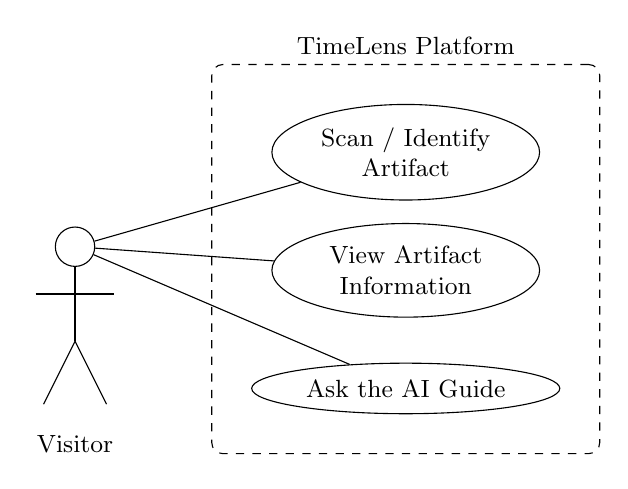
\begin{tikzpicture}[node distance=6mm and 28mm]
  % actor
  \node (head) at (0,0) [circle,draw,minimum size=5mm] {};
  \draw (0,-2.5mm)--(0,-12mm);            % body
  \draw (-5mm,-6mm)--(5mm,-6mm);          % arms
  \draw (0,-12mm)--(-4mm,-20mm);          % legs
  \draw (0,-12mm)--(4mm,-20mm);
  \node (visitor) at (0,-2.5) {\small Visitor};
  % use cases
  \node[draw,ellipse,align=center,minimum width=34mm,font=\small] (scan) at (4.2,1.2) {Scan / Identify\\ Artifact};
  \node[draw,ellipse,align=center,minimum width=34mm,font=\small] (info) at (4.2,-0.3) {View Artifact\\ Information};
  \node[draw,ellipse,align=center,minimum width=34mm,font=\small] (chat) at (4.2,-1.8) {Ask the AI Guide};
  % system boundary
  \begin{scope}[on background layer]
    \node[draw,dashed,rounded corners,fit=(scan)(info)(chat),inner sep=5mm,label=above:{\small TimeLens Platform}] {};
  \end{scope}
  % associations
  \draw (head) -- (scan);
  \draw (head) -- (info);
  \draw (head) -- (chat);
\end{tikzpicture}
\caption{Primary use cases for visitor interaction.}
\label{fig:usecase}
\end{figure}

\FloatBarrier

\section{Interaction and Data Modeling}

System interactions are organized by actor role. Data modeling focuses on the
alignment of user sessions, artifact scans, and bilingual content, ensuring
consistency between the on-device layer and the knowledge backend.

\section{Requirements Traceability Matrix}

Table~\ref{tab:traceability} maps a representative subset of requirements to the
components that satisfy them and the method used to validate each.

\begin{table}[htbp]
\centering\small
\caption{Requirement-to-component mapping.}
\label{tab:traceability}
\begin{tabularx}{\textwidth}{@{}l>{\raggedright\arraybackslash}X>{\raggedright\arraybackslash}X>{\raggedright\arraybackslash}p{2.3cm}@{}}
\toprule
\textbf{Req.} & \textbf{Description} & \textbf{Component} & \textbf{Validation}\\
\midrule
FR-01 & Live detection $+$ tracking overlay & ARService $+$ TFLiteService (YOLOv8n) & Functional test\\
FR-02 & On-device 51-class classification & TFLiteService (end-to-end NMS) & Per-class mAP eval\\
FR-03 & Confident $\rightarrow$ info; sub-threshold $\rightarrow$ suppressed & Home / Scanning logic & End-to-end scenario\\
FR-05 & Bilingual grounded AI guide & RAG \texttt{/ask} (ChromaDB $+$ Gemma) $+$ ChatDrawer & API integration\\
FR-06 & EN/AR switch $+$ RTL $+$ persistence & LocaleController $+$ l10n & UI test (both locales)\\
FR-07 & Text-to-speech replies & \texttt{flutter\_tts} (ChatDrawer) & Functional test\\
NFR-2 & Compact model $\leq 8$\,MB & YOLOv8n TFLite FP16 (5.97\,MB) & Asset-size check\\
NFR-4 & On-device privacy / local backend & On-device inference $+$ local Ollama & Architecture review\\
\bottomrule
\end{tabularx}
\end{table}

\chapter{System Architecture and Design}

\section{High-Level Architecture}

The architecture is intentionally split into two layers with a clear boundary. On the
phone, an \emph{on-device perception layer} turns each camera frame into a tracked,
classified artifact. A \emph{knowledge layer} then grounds any follow-up question in
curated museum data before a language model phrases the answer. This framing avoids a
common failure mode in heritage systems, where a single weak prediction directly
triggers a confident generated answer.

At the system level, \TimeLens{} separates concerns across five layers: experience,
on-device detection, knowledge and retrieval, service, and data. Each layer can evolve
independently behind a stable contract: the detector can be retrained, the knowledge
base updated, or the language model swapped, without collapsing the end-to-end journey.

\section{High-Level System Block Diagram}

Figure~\ref{fig:block} shows how the two layers connect at runtime. Detection runs
entirely on the phone; only a chat question crosses the network, reaching the FastAPI
service that retrieves from ChromaDB and prompts the locally served Gemma model.

\begin{figure}[htbp]
\centering
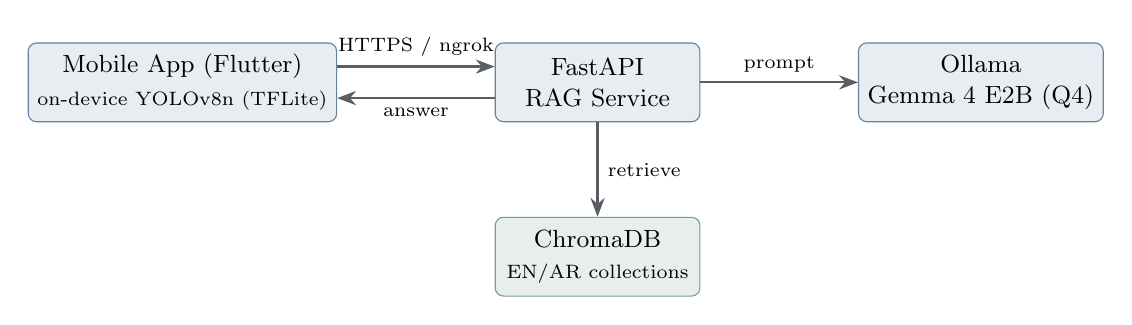
\begin{tikzpicture}[node distance=12mm and 20mm]
  \node[block] (app) {Mobile App (Flutter)\\[1pt]\scriptsize on-device YOLOv8n (TFLite)};
  \node[block,right=of app] (api) {FastAPI\\ RAG Service};
  \node[block,right=of api] (gemma) {Ollama\\ Gemma 4 E2B (Q4)};
  \node[store,below=of api] (chroma) {ChromaDB\\\scriptsize EN/AR collections};
  \draw[flow] ([yshift=2mm]app.east) -- node[above,font=\scriptsize]{HTTPS / ngrok} ([yshift=2mm]api.west);
  \draw[flow] ([yshift=-2mm]api.west) -- node[below,font=\scriptsize]{answer} ([yshift=-2mm]app.east);
  \draw[flow] (api) -- node[above,font=\scriptsize]{prompt} (gemma);
  \draw[flow] (api) -- node[right,font=\scriptsize]{retrieve} (chroma);
\end{tikzpicture}
\caption{System block diagram: detection runs on-device; only chat questions reach the
FastAPI RAG service, which retrieves from ChromaDB and prompts a locally served Gemma
model.}
\label{fig:block}
\end{figure}

\FloatBarrier

\section{Layered System Architecture}

Viewed as layers (Figure~\ref{fig:layers}), the separation of concerns becomes
explicit. The experience layer fans out into two independent paths: an
\emph{on-device path}, where detection resolves artifact identity and metadata
with no network dependency, and a \emph{service path}, where a chat question
crosses HTTPS/ngrok once to the FastAPI endpoints fronting the knowledge layer.
Each boundary is a stable contract, and both paths terminate in the same
canonical dataset, so \emph{grounding}---constraining generation to retrieved
museum data---holds by construction.

\begin{figure}[htbp]
\centering
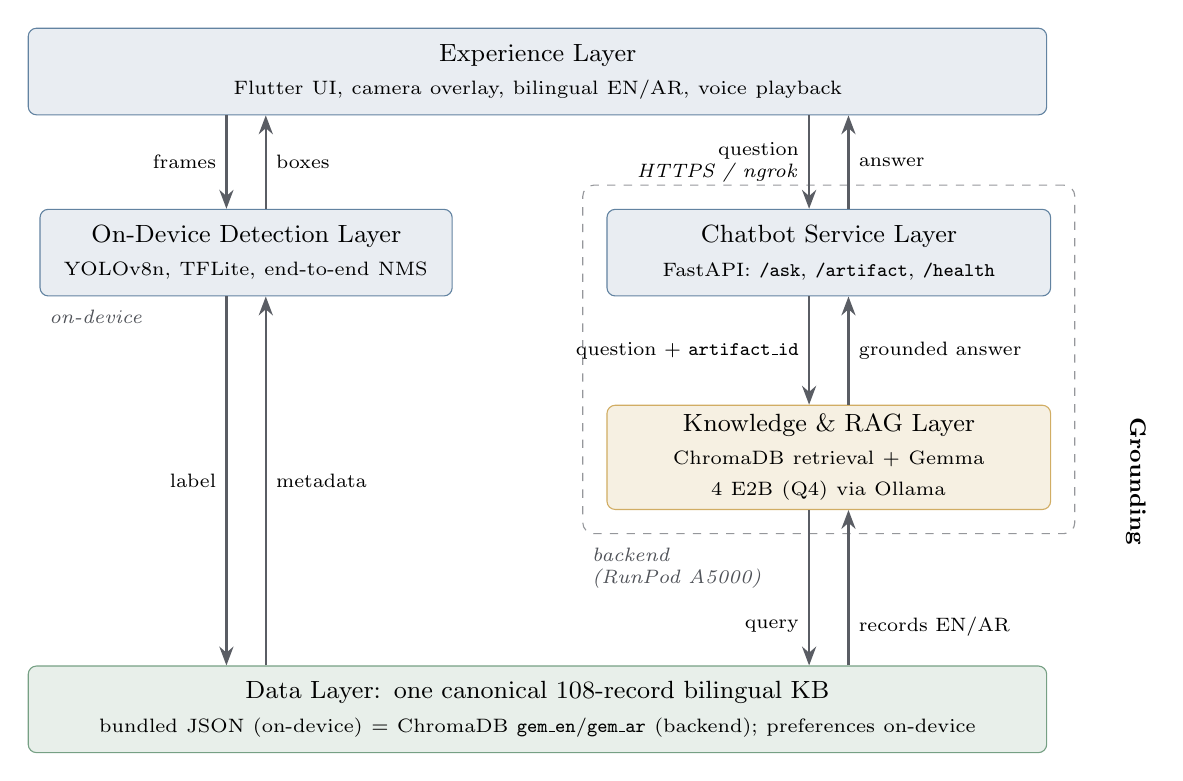
\begin{tikzpicture}[every node/.style={font=\small}]
  % column layers
  \node[block,text width=50mm,minimum height=11mm] (det) at (0,0)
    {On-Device Detection Layer\\[1pt]\scriptsize YOLOv8n, TFLite, end-to-end NMS};
  \node[block,text width=54mm,minimum height=11mm] (svc) at (7.4,0)
    {Chatbot Service Layer\\[1pt]\scriptsize FastAPI: \texttt{/ask}, \texttt{/artifact}, \texttt{/health}};
  \node[edgenode,text width=54mm,minimum height=11mm] (rag) at (7.4,-2.6)
    {Knowledge \& RAG Layer\\[1pt]\scriptsize ChromaDB retrieval $+$ Gemma 4 E2B (Q4) via Ollama};
  % spanning layers
  \node[block,text width=127mm,minimum height=11mm] (exp) at (3.7,2.3)
    {Experience Layer\\[1pt]\scriptsize Flutter UI, camera overlay, bilingual EN/AR, voice playback};
  \node[store,text width=127mm,minimum height=11mm] (data) at (3.7,-5.8)
    {Data Layer: one canonical 108-record bilingual KB\\[1pt]\scriptsize
     bundled JSON (on-device) $=$ ChromaDB \texttt{gem\_en}/\texttt{gem\_ar} (backend);
     preferences on-device};
  % backend boundary
  \begin{scope}[on background layer]
    \node[draw=gemobsidian!45,dashed,rounded corners=4pt,inner sep=3mm,
          fit=(svc)(rag)] (bk) {};
  \end{scope}
  \node[font=\scriptsize\itshape,text=gemobsidian!75,anchor=north west,align=left]
    at ([yshift=-0.5mm]bk.south west) {backend\\(RunPod A5000)};
  \node[font=\scriptsize\itshape,text=gemobsidian!75,anchor=north west]
    at ([yshift=-0.5mm]det.south west) {on-device};
  % layer contracts: requests flow down, responses flow up
  \draw[flow] ($(exp.south -| det)+(-2.5mm,0)$) -- node[left,font=\scriptsize]{frames}
              ($(det.north)+(-2.5mm,0)$);
  \draw[flow] ($(det.north)+(2.5mm,0)$) -- node[right,font=\scriptsize]{boxes}
              ($(exp.south -| det)+(2.5mm,0)$);
  \draw[flow] ($(exp.south -| svc)+(-2.5mm,0)$) -- node[left,align=right,font=\scriptsize]
              {question\\ \textit{HTTPS / ngrok}} ($(svc.north)+(-2.5mm,0)$);
  \draw[flow] ($(svc.north)+(2.5mm,0)$) -- node[right,font=\scriptsize]{answer}
              ($(exp.south -| svc)+(2.5mm,0)$);
  \draw[flow] ($(det.south)+(-2.5mm,0)$) -- node[left,font=\scriptsize]{label}
              ($(data.north -| det)+(-2.5mm,0)$);
  \draw[flow] ($(data.north -| det)+(2.5mm,0)$) -- node[right,font=\scriptsize]{metadata}
              ($(det.south)+(2.5mm,0)$);
  \draw[flow] ($(svc.south)+(-2.5mm,0)$) -- node[left,font=\scriptsize]
              {question $+$ \texttt{artifact\_id}} ($(rag.north)+(-2.5mm,0)$);
  \draw[flow] ($(rag.north)+(2.5mm,0)$) -- node[right,font=\scriptsize]{grounded answer}
              ($(svc.south)+(2.5mm,0)$);
  \draw[flow] ($(rag.south)+(-2.5mm,0)$) -- node[left,font=\scriptsize,pos=0.75]{query}
              ($(data.north -| rag)+(-2.5mm,0)$);
  \draw[flow] ($(data.north -| rag)+(2.5mm,0)$) -- node[right,font=\scriptsize,pos=0.25]{records EN/AR}
              ($(rag.south)+(2.5mm,0)$);
  % grounding guarantee on the generative path
  \node[rotate=-90,anchor=center,font=\footnotesize\bfseries]
    at (11.3,-2.9) {Grounding};
\end{tikzpicture}
\caption{Layered architecture. Downward arrows carry requests, upward arrows the
responses. The experience layer fans out into two independent
paths: detection and metadata lookup resolve entirely on-device, while a chat
question crosses the network once (HTTPS/ngrok) to the FastAPI service fronting
the RAG engine. Both paths draw on the same canonical 108-record bilingual
dataset---bundled as JSON on the device, indexed as ChromaDB collections on the
backend---and ``grounding'' constrains generation to that retrieved museum data.}
\label{fig:layers}
\end{figure}

\FloatBarrier

\subsection{Class Design}

Figure~\ref{fig:classdesign} sketches the core classes behind this flow. The mobile
client drives an on-device \texttt{TFLiteDetector}, resolves artifact metadata locally,
and calls the bilingual \texttt{RagService} only for chat---there is no backend ensemble
verifier in the deployed path.

\begin{figure}[htbp]
\centering
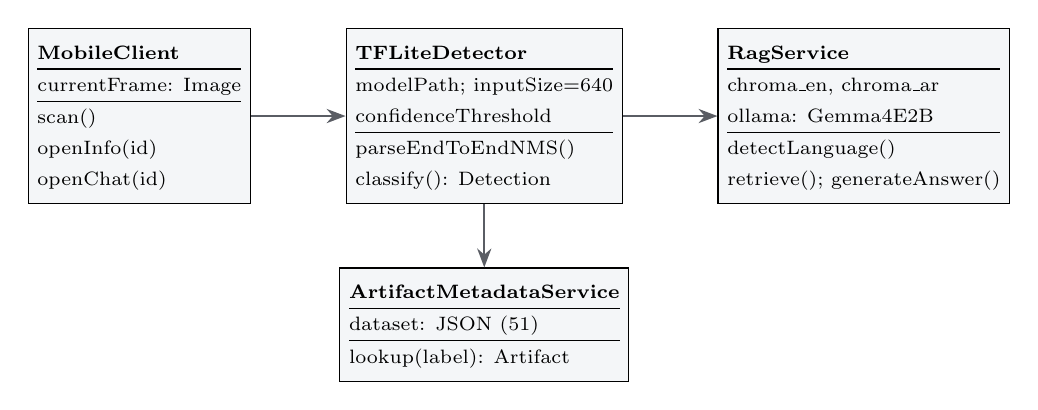
\begin{tikzpicture}[node distance=8mm and 12mm,cls/.style={draw,fill=gemblue!5,font=\scriptsize,align=left}]
  \node[cls] (client) {\begin{tabular}{@{}l@{}}\textbf{MobileClient}\\\hline currentFrame: Image\\\hline scan()\\ openInfo(id)\\ openChat(id)\end{tabular}};
  \node[cls,right=of client] (det) {\begin{tabular}{@{}l@{}}\textbf{TFLiteDetector}\\\hline modelPath; inputSize=640\\ confidenceThreshold\\\hline parseEndToEndNMS()\\ classify(): Detection\end{tabular}};
  \node[cls,below=of det] (meta) {\begin{tabular}{@{}l@{}}\textbf{ArtifactMetadataService}\\\hline dataset: JSON (51)\\\hline lookup(label): Artifact\end{tabular}};
  \node[cls,right=of det] (rag) {\begin{tabular}{@{}l@{}}\textbf{RagService}\\\hline chroma\_en, chroma\_ar\\ ollama: Gemma4E2B\\\hline detectLanguage()\\ retrieve(); generateAnswer()\end{tabular}};
  \draw[flow] (client) -- (det);
  \draw[flow] (det) -- (meta);
  \draw[flow] (det) -- (rag);
\end{tikzpicture}
\caption{Core class design: on-device detection (\texttt{TFLiteDetector}), local metadata
lookup, and the bilingual RAG service. There is no backend ensemble verifier.}
\label{fig:classdesign}
\end{figure}

\subsection{Scan-to-Answer Sequence}

Figure~\ref{fig:sequence} traces one interaction from end to end. Identity is decided
on-device the moment the visitor frames an artifact; the backend is contacted only when
a question is asked, and only to retrieve context and phrase the answer.

\begin{figure}[htbp]
\centering
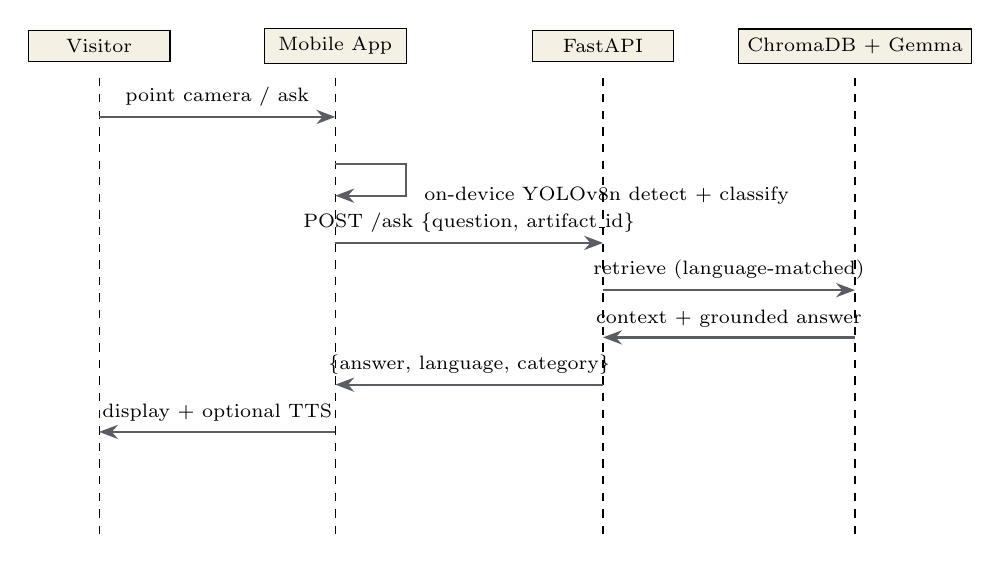
\begin{tikzpicture}[font=\scriptsize]
  \def\ytop{0} \def\ybot{-6.2}
  \foreach \x/\name in {0/Visitor, 3/Mobile App, 6.4/FastAPI, 9.6/{ChromaDB + Gemma}}{
    \node[draw,fill=gemsand,minimum width=18mm] (h\x) at (\x,\ytop) {\name};
    \draw[dashed] (\x,\ytop-0.4) -- (\x,\ybot);
  }
  \draw[flow] (0,-0.9) -- node[above]{point camera / ask} (3,-0.9);
  \draw[flow] (3,-1.5) -- ++(0.9,0) |- (3,-1.9) node[right,xshift=10mm]{on-device YOLOv8n detect + classify};
  \draw[flow] (3,-2.5) -- node[above]{POST /ask \{question, artifact\_id\}} (6.4,-2.5);
  \draw[flow] (6.4,-3.1) -- node[above]{retrieve (language-matched)} (9.6,-3.1);
  \draw[flow] (9.6,-3.7) -- node[above]{context + grounded answer} (6.4,-3.7);
  \draw[flow] (6.4,-4.3) -- node[above]{\{answer, language, category\}} (3,-4.3);
  \draw[flow] (3,-4.9) -- node[above]{display + optional TTS} (0,-4.9);
\end{tikzpicture}
\caption{End-to-end scan-to-answer sequence. Identity is decided on-device; the backend
only grounds and phrases the answer.}
\label{fig:sequence}
\end{figure}

\section{System Interaction Timeline}

The interaction is governed by an on-device confidence gate followed by
retrieval-based factual grounding. Every step, from camera capture to the final
answer, is designed so that the language model is invoked only after an artifact
identity is established and only with retrieved, verified context.

\section{Operational Pipeline}

The deployed behavior is supported by a small set of operational modules on the
knowledge side. Rather than a fabricated ``self-healing'' pipeline, these are the real
scripts that build and serve the bilingual knowledge base
(Table~\ref{tab:ragmodules}).

\begin{table}[htbp]
\centering
\caption{Operational modules of the RAG knowledge service.}
\label{tab:ragmodules}
\begin{tabularx}{\textwidth}{@{}llX@{}}
\toprule
\textbf{Stage} & \textbf{Module} & \textbf{Responsibility}\\
\midrule
Dataset cleaning      & \texttt{clean\_dataset.py} & Normalize fields (e.g., strip a stray ``pigment'' prefix from a location).\\
Loading / chunking    & \texttt{load\_dataset.py}  & Split each record into identity / description / significance chunks.\\
Indexing              & \texttt{index\_dataset.py} & Build the language-separated EN/AR ChromaDB collections (215 chunks).\\
Model serving         & \texttt{load\_model.py}    & Load Gemma 4 E2B via Ollama (cached; \texttt{keep\_alive}\,$=-1$).\\
Retrieval + generation& \texttt{Rag\_engine.py}    & Language detect, query classify, retrieve, build prompt, generate.\\
API                   & \texttt{api.py}            & FastAPI \texttt{/ask}, \texttt{/ask/stream}, \texttt{/artifact/\{id\}}, \texttt{/health}.\\
\bottomrule
\end{tabularx}
\end{table}

\section{Inference Pipeline Architecture}

On-device recognition follows a fixed, deterministic sequence
(Figure~\ref{fig:infpipeline}). Each camera frame arrives as sensor-rotated YUV420
data, which is converted to RGB, rotated $90^{\circ}$ to match the Android sensor
orientation, resized to $640\times640$, and normalized before inference. The YOLOv8n
model is exported with non-maximum suppression baked in, so a single forward pass
returns a fixed-size \texttt{[1,300,6]} tensor of \texttt{(xyxy, score, class)} rows
rather than raw anchors, removing any post-processing decode step on the device. A
confidence and geometry filter (global threshold $0.75$, raised to $0.90$ for the
visually near-identical Statue of Siptah) then keeps only trustworthy detections, which
are tracked and drawn as overlays; tapping one opens the artifact's information and the
RAG chat. Running NMS inside the model keeps per-frame latency at roughly
30--60\,ms on a mid-tier Android phone.

\begin{figure}[htbp]
\centering
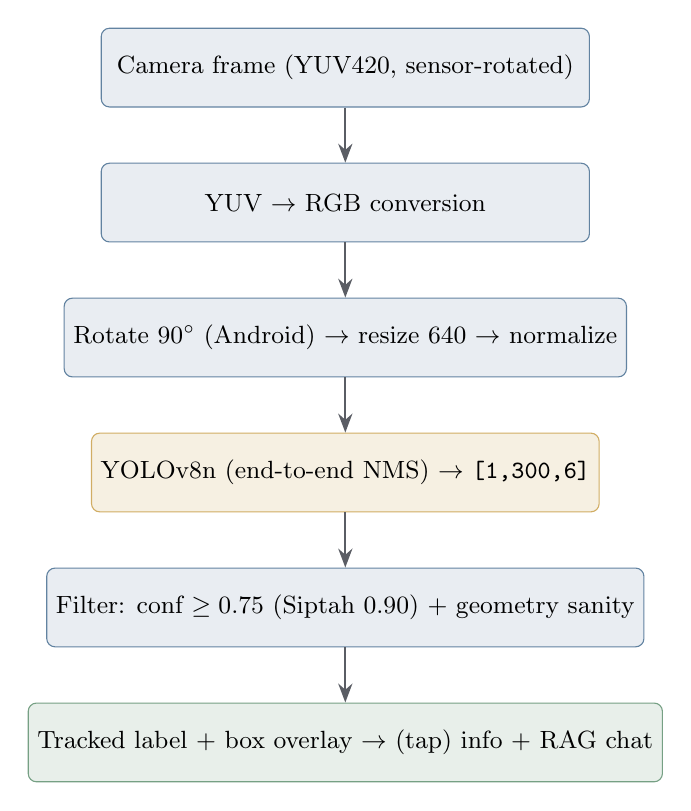
\begin{tikzpicture}[node distance=7mm,every node/.style={font=\small}]
  \node[block,minimum width=62mm] (a) {Camera frame (YUV420, sensor-rotated)};
  \node[block,minimum width=62mm,below=of a] (b) {YUV $\rightarrow$ RGB conversion};
  \node[block,minimum width=62mm,below=of b] (c) {Rotate $90^{\circ}$ (Android) $\rightarrow$ resize $640$ $\rightarrow$ normalize};
  \node[edgenode,minimum width=62mm,below=of c] (d) {YOLOv8n (end-to-end NMS) $\rightarrow$ \texttt{[1,300,6]}};
  \node[block,minimum width=62mm,below=of d] (e) {Filter: conf $\geq 0.75$ (Siptah $0.90$) $+$ geometry sanity};
  \node[store,minimum width=62mm,below=of e] (f) {Tracked label + box overlay $\rightarrow$ (tap) info + RAG chat};
  \foreach \x/\y in {a/b,b/c,c/d,d/e,e/f}{\draw[flow] (\x) -- (\y);}
\end{tikzpicture}
\caption{On-device inference pipeline from raw camera frame to a tracked, classified
artifact. Non-maximum suppression is baked into the exported model.}
\label{fig:infpipeline}
\end{figure}


\section{Data Flow Architecture}

The information lifecycle is a progressive journey from a raw scan to a grounded
answer: detect on-device, look up local metadata, and---only when the visitor
asks---retrieve bilingual context and generate a response. No camera frames leave the
device, and no per-frame data is logged remotely.

\section{Technology Stack Selection}

\begin{itemize}[leftmargin=1.5em]
  \item \textbf{Mobile app:} Flutter with Provider state management.
  \item \textbf{On-device detection:} YOLOv8n (Ultralytics) exported to TensorFlow Lite
        (FP16) with end-to-end NMS.
  \item \textbf{RAG backend:} FastAPI $+$ LlamaIndex $+$ LangChain; Ollama serving
        Gemma 4 E2B (Q4\_K\_M); ChromaDB vector store; multilingual MiniLM embeddings.
  \item \textbf{Detector training:} Ultralytics 8.4.45 / PyTorch; YOLO-World for
        auto-annotation; Roboflow for hand annotation.
  \item \textbf{Serving / infrastructure:} RunPod-hosted NVIDIA RTX A5000
        (24\,GB VRAM) exposed via an ngrok tunnel.
\end{itemize}

\section{Gemma Integration and Grounding}

Gemma is intentionally downstream of identity. The system never asks Gemma to decide
which artifact is in view; identity is established by the calibrated on-device
detector. Gemma is asked only to narrate \emph{retrieved} museum context after an
artifact is known. This grounding contract keeps the language layer aligned with
museum-safe behavior: if the relevant facts are not in the retrieved context, the
model is instructed to say so rather than invent them. Backend re-verification of the
on-device label is supported by the architecture but is not required in the deployed
path.

\section{Production Deployment Strategy}

The deployment defines clear boundaries between the mobile edge (on-device detection
and UI) and the knowledge backend (FastAPI RAG on a RunPod RTX A5000, exposed via ngrok).
This separation keeps the visitor-facing experience responsive and lets the knowledge
base and model evolve without an app release.

\section{App UI and UX Design Integration}

UI and UX were treated as part of system reliability. The app is designed so that user
trust and cognitive load remain stable while model confidence changes in the
background. Instead of exposing raw uncertainty, the navigation guides visitors through
understandable modes: scan, details, contextual learning, and optional conversation.

\section{UI/UX Design Philosophy}

The design philosophy centers on visitor trust. By mapping the operational steps from
visual capture to grounded answer, the system creates a seamless educational journey,
and the hierarchical arrangement of screens lets visitors move naturally between
discovery, scanning, and interactive chat.

\chapter{On-Device Artifact Detection}

\section{Overview}

This chapter presents the on-device detector that powers \TimeLens{}: a compact
YOLOv8n model that recognizes 51 \GEM{} artifacts in real time on a phone. The central
finding is that, for this fine-grained domain, \textbf{label quality dominates model
architecture and input resolution}. We reach a deployable detector not by enlarging
the network but by progressively improving the training labels, from foundation-model
auto-annotation through spatial cleaning rules to full hand annotation.

\section{Problem and Constraints}

Pointing a phone at an exhibit must (i) detect that an artifact is present, (ii)
classify it as one of 51 catalogued artifacts, and (iii) track it with a bounding box
in real time. Deployment constraints rule out cloud detectors: inference must run
on-device (no per-frame round-trip), in real time ($\geq 2.5$\,FPS on mid-tier
phones), with a compact model ($<8$\,MB TFLite asset), and be robust to handheld
capture. These constraints led to YOLOv8-nano with FP16 TensorFlow Lite
deployment~\citep{yolov8,ipalakova2025comparative}.

\section{Objectives and Contributions}

\begin{itemize}[leftmargin=1.5em]
  \item A foundation-model auto-annotation pipeline (YOLO-World) plus four spatial
        sanity rules that recover most labeling failures without manual work.
  \item A controlled iteration study (v1$\rightarrow$v3) that isolates label quality
        from architecture and resolution.
  \item An honest analysis of validation frame leakage and training-to-deployment
        domain shift.
  \item A deployable 5.97\,MB TFLite detector with end-to-end NMS.
\end{itemize}

\section{Methodology}

\subsection{Dataset and Acquisition}
The source material is roughly 50 videos of GEM artifacts captured before public
opening. Frames extracted at about one per second yield approximately 30{,}000
candidate images across 51 classes. Manual annotation of 30k images is infeasible for
a student team, motivating an auto-annotation-first pipeline.

\subsection{v1 --- Auto-Annotated Baseline}
The first labels were produced by YOLO-World (\texttt{yolov8s-worldv2})\citep{yoloworld},
a text-prompted open-vocabulary detector. Each class received a prompt (e.g., ``statue
of Ramesses II'', ``stone stela''), and the highest-confidence box per frame was kept
as ground truth. A YOLOv8n model trained on these labels at $320\times320$ reached
mAP@0.5 $=0.751$, but per-class analysis revealed \textbf{ten classes below mAP@0.5
$=0.30$}. Inspection showed two failure modes: \emph{Mode A} (nine classes), where
YOLO-World boxed the wrong object in the frame (a wall card, a bench, a neighboring
statue); and \emph{Mode B} (one class, \emph{Head of Ramesses III}), sibling-class
confusion between a bust and full-body statues. The architecture was capable; the
labels were the bottleneck.

\subsection{v2 --- Spatial Sanity Rules}
A second-pass annotator added four geometric rules to the YOLO-World output:
(1)~restrict the ``stela'' prompt to the two true stela classes; (2)~drop boxes whose
center lies in the bottom quarter of the frame ($c_y>0.75$), which are almost always
floor signs or bystanders; (3)~pick the largest-area box rather than the
highest-confidence one (artifacts dominate the frame; spurious text boxes are small);
and (4)~for each video, drop boxes whose center deviates from the per-video median by
more than $0.20$. These rules dropped about $6.9\%$ of frames, leaving $27{,}134$.
Retraining (still $320\times320$) raised mAP@0.5 to $0.867$ ($+0.116$ from a labeling
change alone) and reduced broken classes from ten to three. Three classes remained at
zero because their auto-labels were unrecoverable.

\subsection{v2 at 640 and End-to-End NMS}
Raising the input to $640\times640$ and exporting with end-to-end NMS
(\texttt{nms=True}, output \texttt{[1,300,6]}) left mAP@0.5 unchanged at $0.867$ but
lifted mAP@0.5:0.95 from $0.586$ to $0.777$ ($+0.191$): higher resolution improves
\emph{localization} but cannot fix classes whose labels are wrong. The data-quality
ceiling was unmistakable.

\subsection{v3 --- Full Hand Annotation}
All 51 classes were re-annotated by hand in Roboflow ($24{,}384$ images,
$70/20/10$ split), drawing full-artifact boxes, avoiding peripheral objects, and
carefully distinguishing similar artifacts. Warm-started from the v2@640 weights and
trained for 100 epochs on a GTX~1650~Ti, v3 reached precision $0.998$, recall $1.000$,
mAP@0.5 $0.995$, and mAP@0.5:0.95 $0.924$, with \textbf{zero broken classes}. The
validation classification loss collapsed from $0.892$ to $0.166$ --- the model's
quantitative way of saying the labels are now internally consistent.

\section{Core Algorithms}

Two procedures capture the steps most prone to error. The first formalizes the
auto-annotation pass and its spatial sanity rules (the v1$\rightarrow$v2 transition);
the second shows how the exported model's end-to-end NMS output is parsed and
deduplicated on-device.

\begin{algorithm}[htbp]
\caption{Auto-annotation with spatial sanity rules (v1$\rightarrow$v2)}
\KwIn{video frames $F$; per-class text prompts $P$; true-stela class set $S$}
\KwOut{one labeled box per usable frame}
\ForEach{frame $f \in F$ (class $c$ from its folder)}{
  $B \leftarrow \textsc{YoloWorld}(f, P)$\;
  \If{$c \notin S$}{remove stela-prompt detections from $B$}
  remove boxes with center $c_y > 0.75$\;
  \If{$B \neq \emptyset$}{
    $b^\star \leftarrow \arg\max_{b\in B}\;\mathrm{area}(b)$ \tcp*{tie-break on confidence}
    drop $b^\star$ if its center deviates $>0.20$ from the per-video median center\;
    \If{$b^\star$ kept}{emit $(b^\star, c)$}
  }
}
\end{algorithm}

\begin{algorithm}[htbp]
\caption{On-device parsing of end-to-end NMS output (with same-class dedup)}
\KwIn{model output $T$ of shape \texttt{[1,300,6]}; per-class thresholds $\tau(\cdot)$}
\KwOut{deduplicated detections $D$}
$D \leftarrow \emptyset$\;
\ForEach{row $r=(x_1,y_1,x_2,y_2,\mathit{conf},\mathit{cls}) \in T$}{
  \If{$\mathit{conf} \geq \tau(\mathit{cls})$ \textbf{and} box geometry is valid}{
    $c \leftarrow$ center of $r$\;
    \If{some kept $r' \in D$ has class $\mathit{cls}$ and contains $c$}{
      replace $r'$ with $r$ if $\mathrm{conf}(r) > \mathrm{conf}(r')$ \tcp*{in-graph NMS leaks identical rows; dedup required}
    }
    \Else{add $r$ to $D$}
  }
}
\Return $D$\;
\end{algorithm}

\section{Experimental Design}

Detection quality is measured with the standard object-detection metrics. With true
positives (TP), false positives (FP), and false negatives (FN), and predicted/ground-truth
boxes $A,B$:
\begin{equation}\mathrm{IoU}(A,B)=\frac{|A\cap B|}{|A\cup B|}\end{equation}
\begin{equation}\mathrm{Precision}=\frac{\mathrm{TP}}{\mathrm{TP}+\mathrm{FP}}\end{equation}
\begin{equation}\mathrm{Recall}=\frac{\mathrm{TP}}{\mathrm{TP}+\mathrm{FN}}\end{equation}
\begin{equation}\mathrm{AP}=\int_{0}^{1} p(r)\,\mathrm{d}r\end{equation}
\begin{equation}\mathrm{mAP}=\frac{1}{N}\sum_{i=1}^{N}\mathrm{AP}_i\end{equation}
where $p(r)$ is the precision--recall curve and AP its area; mAP@0.5 evaluates at
IoU $=0.5$ and mAP@0.5:0.95 averages AP over IoU thresholds $0.5,0.55,\dots,0.95$. We
also report the number of \emph{broken} classes (mAP@0.5 $<0.30$), since per-class
failure matters more than the average for a visitor-facing app.

\section{Results and Analysis}

Table~\ref{tab:iteration} summarizes the four iterations and Figure~\ref{fig:iteration}
plots the mAP@0.5 progression. The dominant lesson is that label cleaning ($+0.116$
mAP@0.5, no model change) and hand annotation ($+0.128$ mAP@0.5, $+0.147$ mAP@0.5:0.95)
broke ceilings that resolution scaling could not.

\begin{table}[htbp]
\centering\small
\setlength{\tabcolsep}{5pt}
\caption{Detector iteration comparison (validation).}
\label{tab:iteration}
\begin{tabular}{@{}lllllll@{}}
\toprule
\textbf{Iter.} & \textbf{Labels} & \textbf{imgsz} & \textbf{Head} & \textbf{mAP$_{50}$} & \textbf{mAP$_{50:95}$} & \textbf{Broken}\\
\midrule
v1     & Auto (YOLO-World)       & 320 & raw     & 0.751 & ---   & 10\\
v2     & Auto $+$ 4 rules        & 320 & raw     & 0.867 & 0.586 & 3\\
v2@640 & Auto $+$ rules          & 640 & E2E NMS & 0.867 & 0.777 & 3\\
\textbf{v3} & \textbf{Hand-annotated} & \textbf{640} & \textbf{E2E NMS} & \textbf{0.995} & \textbf{0.924} & \textbf{0}\\
\bottomrule
\end{tabular}
\end{table}

\begin{figure}[htbp]
\centering
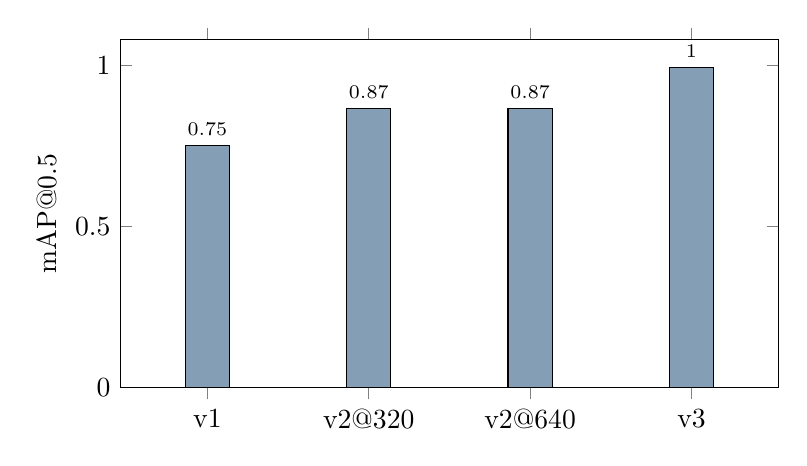
\begin{tikzpicture}
\begin{axis}[ybar,symbolic x coords={v1,v2@320,v2@640,v3},xtick=data,
  ymin=0,ymax=1.08,ylabel={mAP@0.5},bar width=16pt,width=0.82\textwidth,height=6cm,
  nodes near coords,every node near coord/.append style={font=\scriptsize},
  enlarge x limits=0.18]
\addplot[fill=gemblue!55] coordinates {(v1,0.751)(v2@320,0.867)(v2@640,0.867)(v3,0.995)};
\end{axis}
\end{tikzpicture}
\caption{Detection mAP@0.5 across iterations: label cleaning (v1$\rightarrow$v2) and
hand annotation (v2@640$\rightarrow$v3) drive the gains; resolution scaling alone leaves
mAP@0.5 flat.}
\label{fig:iteration}
\end{figure}

Hand annotation rescued every previously broken class
(Table~\ref{tab:rescue}). Figure~\ref{fig:detexample} shows live detections from the
deployed app, including the Amenhotep~II / Thutmose~III sibling pair distinguished
simultaneously.

\begin{table}[htbp]
\centering
\caption{Per-class rescue from auto-labels (v2) to hand-labels (v3), mAP@0.5:0.95.}
\label{tab:rescue}
\begin{tabular}{@{}lcc@{}}
\toprule
\textbf{Class} & \textbf{v2} & \textbf{v3}\\
\midrule
Double Statue of Ramesses II        & 0.000 & 0.995\\
Overseer Amenemhat                  & 0.000 & 0.940\\
Thutmose III Statue                 & 0.000 & 0.941\\
Naktmin and Tiy                     & 0.269 & 0.977\\
Statue of King Akhenaten            & 0.281 & 0.955\\
Seated Statue of King Thutmose III  & 0.440 & 0.862\\
\bottomrule
\end{tabular}
\end{table}

\begin{figure}[htbp]
\centering
\begin{minipage}{0.40\textwidth}\centering
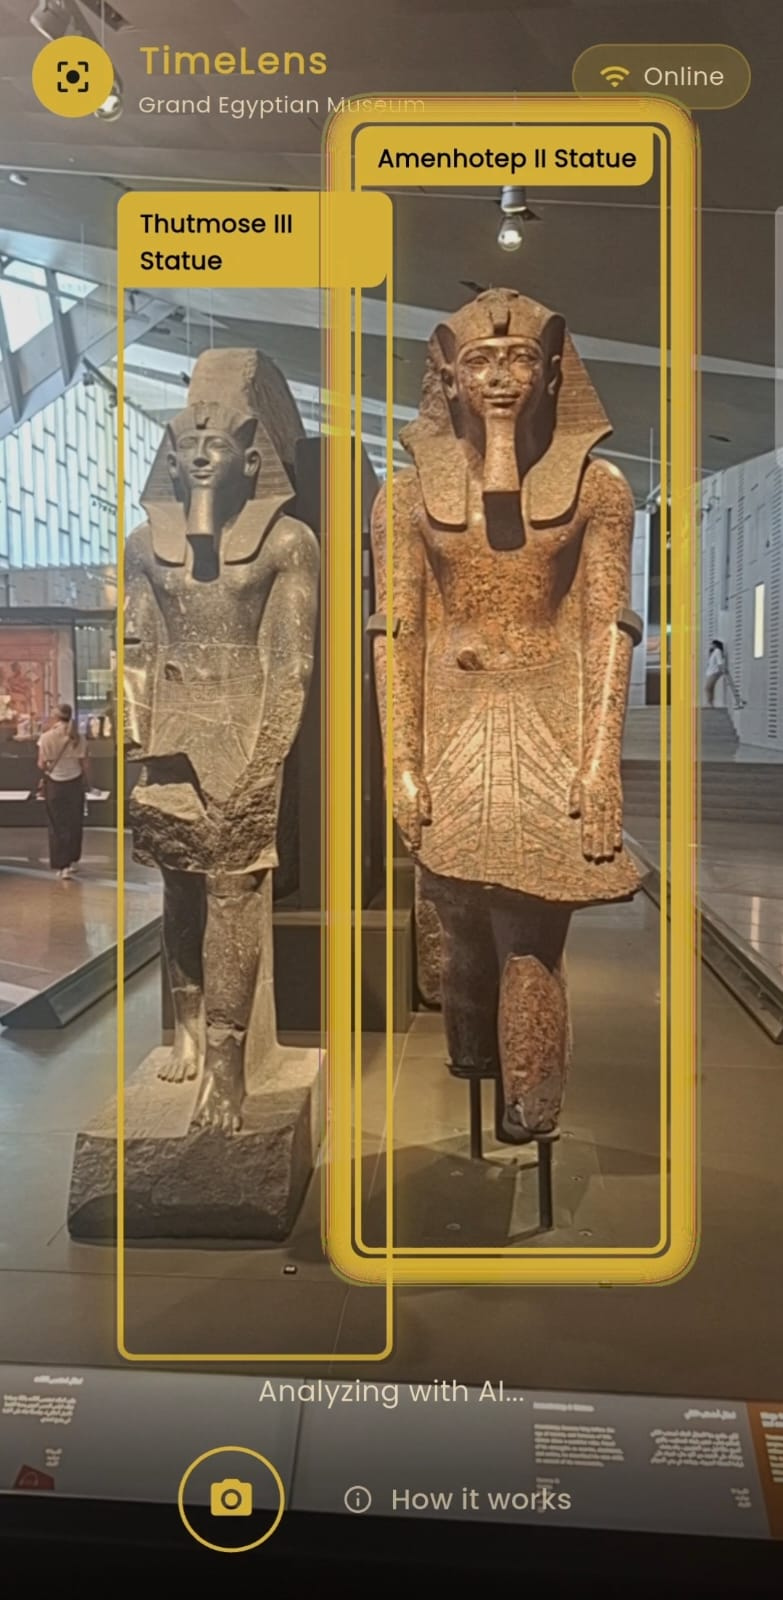
\includegraphics[width=\linewidth]{app_detection_1.jpg}\\[1mm](a)
\end{minipage}\hfill
\begin{minipage}{0.40\textwidth}\centering
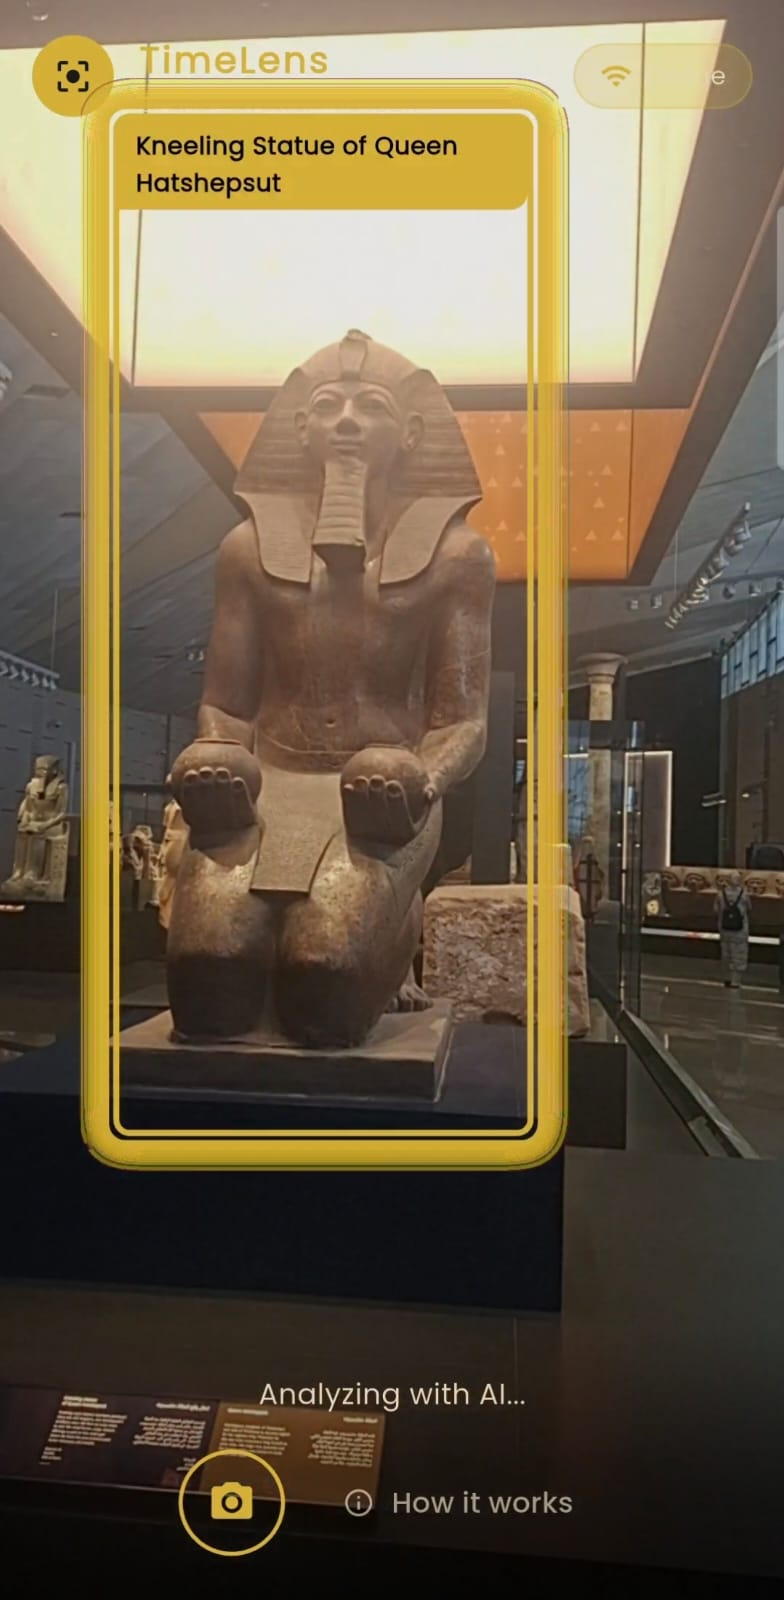
\includegraphics[width=\linewidth]{app_detection_2.jpg}\\[1mm](b)
\end{minipage}
\caption{Live on-device detection in the deployed \TimeLens{} app: (a) two
near-identical New Kingdom statues distinguished at once---Amenhotep~II versus
Thutmose~III, the canonical fine-grained sibling case; (b) the Kneeling Statue of Queen
Hatshepsut. Each box appears only after clearing the on-device confidence gate.}
\label{fig:detexample}
\end{figure}

\section{Failure Modes and Caveats}

The v3 validation metrics \emph{overstate} real-world generalization, and we disclose
this plainly.

\textbf{Frame leakage.} The dataset is video frames split randomly per image. Adjacent
frames are near-duplicates, so a frame in training can have an almost-identical twin in
validation. The v3 mAP@0.5 saturates at $0.995$ within about three epochs of
warm-started training, which is characteristic of memorization rather than
generalization. A conservative, in-distribution \emph{held-out test} (using the
$320$ model) gives a more honest picture: precision $0.691$, recall $0.815$,
mAP@0.5 $0.751$, mAP@0.5:0.95 $0.650$.

\textbf{Domain shift.} Training frames come from stable, pre-opening videos; deployment
uses handheld phone cameras under public lighting with motion blur. Phone-camera
inference is materially worse than on the source videos.

\textbf{Auto-annotation ceiling.} Open-vocabulary detectors handle generic concepts but
fail on fine-grained, domain-specific objects; spatial rules recovered most failures,
but a residual fraction required manual labeling. Figure~\ref{fig:confusion} shows the
residual fine-grained confusion as an off-diagonal structure in the confusion matrix.

\begin{figure}[htbp]
\centering
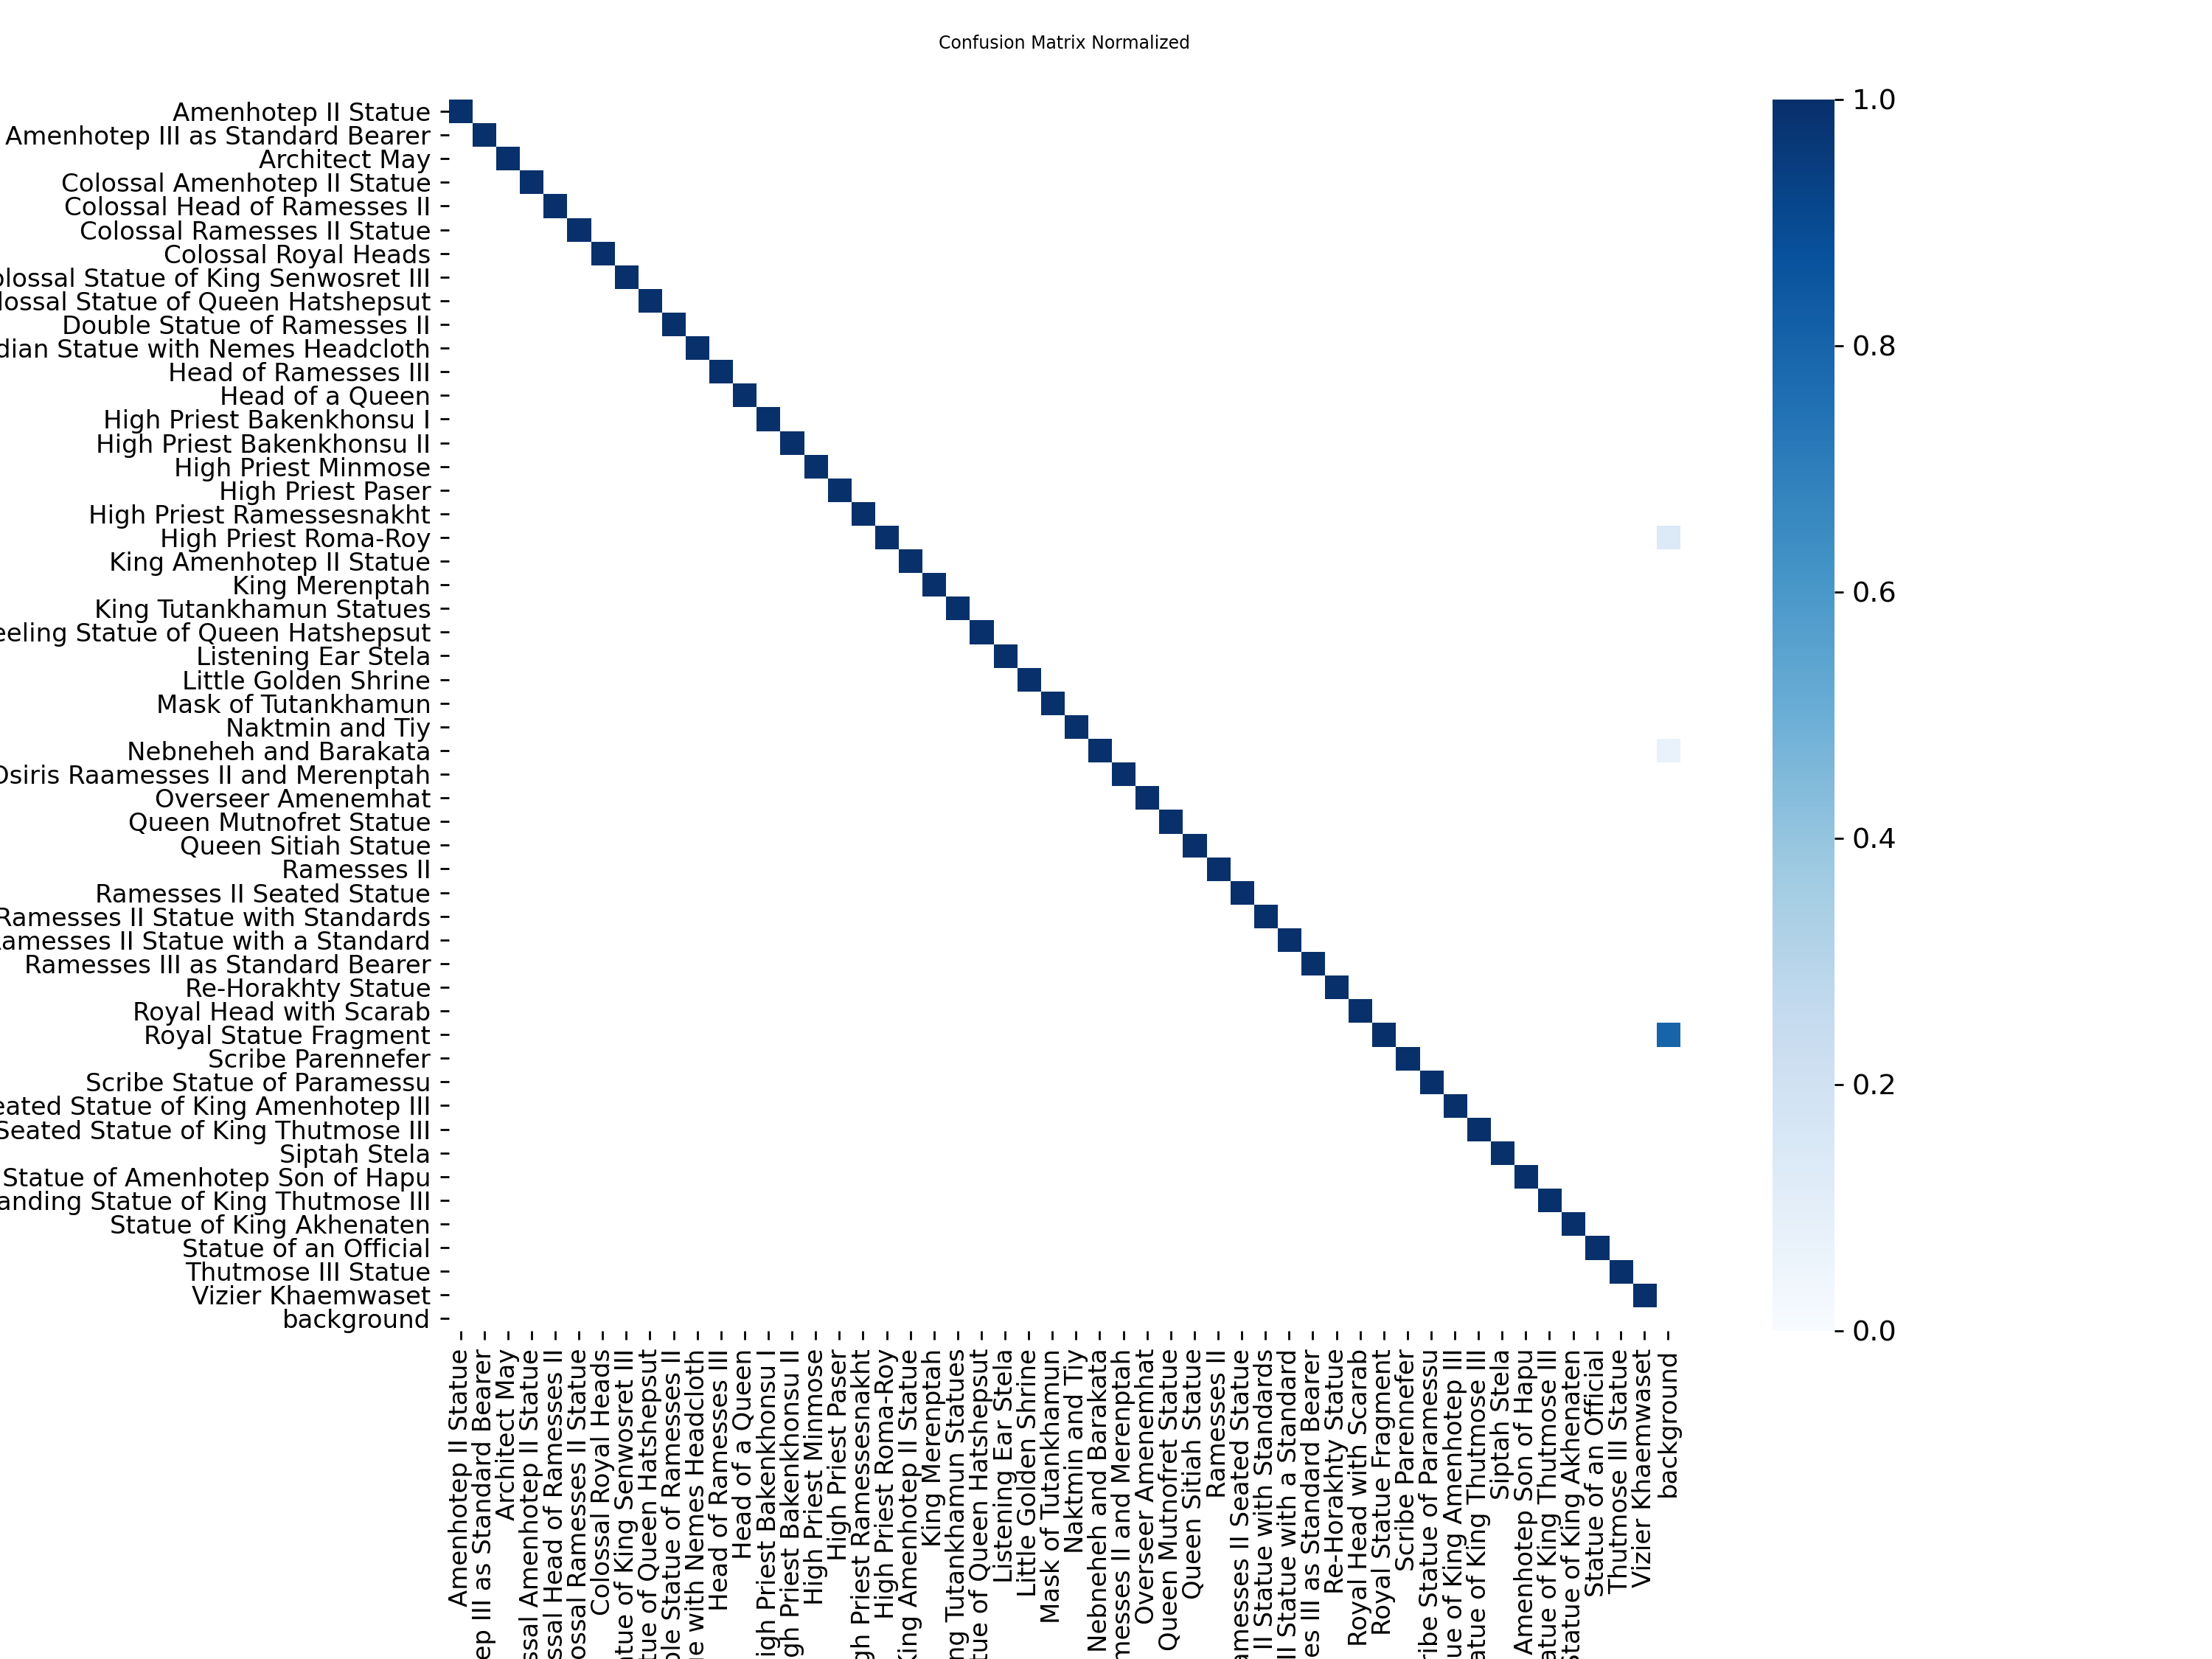
\includegraphics[width=0.82\textwidth]{confusion_matrix.png}
\caption{Normalized 51-class confusion matrix (v3). The strong diagonal confirms
separation; faint off-diagonal cells mark residual sibling-class confusion among
visually similar statues.}
\label{fig:confusion}
\end{figure}

\section{Engineering Findings}

\begin{itemize}[leftmargin=1.5em]
  \item \textbf{Android frame rotation.} Back-camera sensors deliver frames rotated
        $90^{\circ}$ from the display; a rotation step is required before resizing or
        every prediction is computed on a sideways artifact.
  \item \textbf{End-to-end NMS format and duplicate leakage.} The exported output has shape
        \texttt{[1,300,6]}; each row is $(x_1,y_1,x_2,y_2,\mathit{conf},\mathit{cls})$ in
        corner format (not center-width-height), so misreading it stretches and shifts boxes.
        Empirically, the Ultralytics \texttt{nms=True} TFLite export bakes near-zero NMS
        thresholds into the graph, so a single dominant object can produce $100$--$250$
        identical copies of its top-survivor row in the $300$-slot buffer. The on-device
        parser therefore runs a per-class same-center dedup before drawing; without it,
        the overlay would draw the same box over itself many times.
  \item \textbf{Calibration from clean labels.} Clean labels produce sharp confidence
        distributions (real artifacts cluster high; off-target scenes fall well below),
        which lets the app raise its on-device threshold for out-of-distribution
        rejection (global $0.75$, with $0.90$ for the false-positive-prone
        \emph{Siptah Stela}).
  \item \textbf{Footprint.} The deployed asset is FP16 TFLite at \textbf{5.97\,MB},
        running in roughly $30$--$60$\,ms per frame on a mid-tier Android phone.
\end{itemize}

\section{Limitations}

The headline validation metrics are bounded by frame leakage, and a training-to-phone
domain gap remains. The honest, deployment-facing numbers are the held-out test figures
above. Mitigations are deferred to future work (Chapter~8): splitting by video rather
than by frame, capturing a phone-camera deployment test set, and stronger augmentation.

\section{Conclusion}

For fine-grained museum artifacts, \textbf{label quality is first-order}; architecture
and resolution are second-order. A compact YOLOv8n trained on clean, hand-verified
labels yields a deployable, real-time, on-device detector that feeds the rest of the
\TimeLens{} system.

\chapter{Bilingual RAG Museum Guide and Deployment}

\section{Overview}

The conversational guide answers a visitor's questions about an artifact---or about
the museum and ancient Egypt in general---in English or Arabic. It is a
Retrieval-Augmented Generation (RAG) system: rather than relying on a language model's
parametric memory, it retrieves relevant entries from a curated knowledge base and
passes them to the model as grounding context~\citep{lewis2020rag}. The pipeline was
developed in two iterations; this chapter describes both and explains what changed and
why.

\section{Problem and Grounding Principles}

A public museum guide must not invent history. The design therefore follows three
grounding principles: (i)~answers are constrained to retrieved museum context;
(ii)~retrieval is language-matched so an Arabic question receives Arabic context; and
(iii)~when the relevant facts are absent, the model says so rather than fabricating.
Running inference locally (no third-party LLM API) additionally removes per-request
cost and rate limits and keeps visitor queries within a controlled environment.

\section{Knowledge Base}

The knowledge base is a hand-curated set of \textbf{108 records} covering \textbf{54
unique artifacts}, each documented in both English and Arabic. A preprocessing step
fixes data-quality issues---most notably a location field that had absorbed a material
descriptor (reading ``pigment Thebes (Luxor)'' instead of ``Thebes (Luxor)'')---and
preserves the original.

Each record is split into up to three semantically distinct chunks before indexing:
an \emph{identity} chunk (name, material, location, period as discrete facts), a
\emph{description} chunk (appearance and iconography), and a \emph{significance} chunk
(historical and cultural context). The 108 records yield \textbf{215 chunks} (109
English, 106 Arabic). English and Arabic chunks are stored in \emph{separate}
collections (\texttt{\_en} and \texttt{\_ar}); a question is routed only to the
matching collection, eliminating cross-language retrieval confusion.

\section{Retrieval}

Every request begins with language detection: if more than $30\%$ of the question's
characters are Arabic script, it is treated as Arabic, otherwise English. The detected
language selects the collection and the prompt's language instruction.

In \emph{camera mode}, the app sends the English title of the detected artifact and the
retriever performs a deterministic metadata lookup, returning exactly that artifact's
chunks. In \emph{text mode}, a keyword-based query classifier assigns the question to
one of five categories and chooses a strategy accordingly (Table~\ref{tab:querycat}).
Metadata filtering guarantees \emph{completeness} for structured queries (e.g.,
``which artifacts were found at Karnak''), where similarity search would return only
the nearest chunks. A multilingual MiniLM embedding model produces comparable vectors
for English and Arabic, so the same routing serves both languages.

\begin{table}[htbp]
\centering
\caption{Text-mode query categories and retrieval strategy.}
\label{tab:querycat}
\begin{tabularx}{\textwidth}{@{}lX@{}}
\toprule
\textbf{Category} & \textbf{Retrieval strategy}\\
\midrule
Location & Metadata filter on the \texttt{was\_found\_at} field (all matching chunks).\\
Period   & Metadata filter on the historical-overview field.\\
Material & Metadata filter on the material field.\\
Royal    & Similarity search ($k=8$) against the language-matched collection.\\
Generic  & Similarity search ($k=8$) against the language-matched collection.\\
\bottomrule
\end{tabularx}
\end{table}

\section{Generation and Prompting}

The prompt has three parts: system instructions, the retrieved context, and the
question. The model is instructed to act as an Egyptology guide, to use only the
provided context, to write in flowing paragraphs without markdown (the app renders
plain text), and to give at least four sentences. For Arabic questions, the prompt adds
a reference table of the correct Arabic spellings for all fifteen royals in the dataset,
introduced after testing revealed confusions between similarly named rulers
(e.g., the Thutmose and Amenhotep kings). Generation parameters are \texttt{num\_ctx}
$=4096$, \texttt{repeat\_penalty} $=1.3$, \texttt{top\_p} $=0.9$, and
\texttt{temperature} $=0.3$; the model stays resident in GPU memory
(\texttt{keep\_alive} $=-1$). A fallback retry, triggered when a response is too short,
re-issues the prompt with an explicit instruction to answer more completely.

\section{Model Selection}

The generation model was chosen by benchmarking seven candidates against 20
standardized bilingual questions (Table~\ref{tab:funnel}). Four were eliminated:
Gemma~3n~E2B for hallucinating dimensions and locations; the default Gemma~4~E2B for
empty/truncated outputs; Qwen~3~4B because its ``thinking'' mode consumed the entire
token budget; and Qwen~3.5~4B for excessive latency and near-limit VRAM. Among the
three finalists (Table~\ref{tab:finalists}), \textbf{Gemma~4~E2B (Q4\_K\_M)} was
selected: although Llama~3.2~3B is faster, only Gemma~4~E2B~Q4 produced clean,
non-hallucinated answers in \emph{both} English and Arabic, at the lowest cold-start
VRAM.

\begin{table}[htbp]
\centering\small
\setlength{\tabcolsep}{4pt}
\caption{Candidate language models and benchmarking outcome.}
\label{tab:funnel}
\begin{tabular}{@{}lllcl@{}}
\toprule
\textbf{Model} & \textbf{Family} & \textbf{Quant.} & \textbf{VRAM} & \textbf{Verdict}\\
\midrule
Gemma 3n E2B   & Gemma & default & 1349\,MB & Eliminated (hallucination)\\
Gemma 3n E4B   & Gemma & Q3\_K\_M & 2145\,MB & Finalist\\
Gemma 4 E2B    & Gemma & default & 2021\,MB & Eliminated (empty/truncation)\\
\textbf{Gemma 4 E2B} & \textbf{Gemma} & \textbf{Q4\_K\_M} & \textbf{1389--3585\,MB} & \textbf{Selected}\\
Llama 3.2 3B   & Llama & default & 2565\,MB & Finalist\\
Qwen 3 4B      & Qwen  & default & 2907\,MB & Eliminated (thinking-mode)\\
Qwen 3.5 4B    & Qwen  & default & 3485\,MB & Eliminated (latency/VRAM)\\
\bottomrule
\end{tabular}
\end{table}

\begin{table}[htbp]
	\caption{Finalist comparison (pre-optimization).}
	\label{tab:finalists}
\begin{tabularx}{\textwidth}{@{}lXXX@{}}
	\toprule
	\textbf{Criterion} & \textbf{Gemma 3n E4B} & \textbf{Gemma 4 E2B Q4 (selected)} & \textbf{Llama 3.2 3B}\\
	\midrule
Avg.\ speed     & 19.6\,s & 22.7\,s & 7.0\,s\\
English quality & Good (minor additions) & Excellent (grounded) & Excellent (adds external facts)\\
Arabic quality  & Weak (mixed scripts) & Excellent (clean) & Unusable (garbled)\\
Hallucination   & Medium & Low & Medium\\
VRAM            & 2145\,MB & 1389\,MB (cold) & 2565\,MB\\
	\bottomrule
\end{tabularx}
\end{table}

\FloatBarrier
\section{Pipeline Optimizations}
Ten optimizations reduced end-to-end latency from over 30\,s to about 10\,s
(Table~\ref{tab:opts}, Figure~\ref{fig:latency}) while improving answer quality.

\begin{longtable}[c]{@{}>{\raggedright\arraybackslash}p{0.33\textwidth}p{\dimexpr0.67\textwidth-2\tabcolsep\relax}@{}}
	\caption{Pipeline optimizations and measured impact.\label{tab:opts}}\\
%first header
	\hline
	\textbf{Optimization} & \textbf{Measured impact}\\
	\hline
	\endfirsthead
%subsequent headers (spanning across multiple pages)
	\hline
	\textbf{Optimization} & \textbf{Measured impact}\\
	\hline
	\endhead
%subsequent footers
	\hline
	\multicolumn{2}{r}{\footnotesize(To be continued)}
	\endfoot
%end of table
	\hline
	\endlastfoot
Hierarchical chunking
(identity/description/significance)			& Replaced flat documents with semantically distinct chunks, giving the retriever precise targets. Narrow factual questions now return the identity chunk only, eliminating retrieval noise from irrelevant descriptive content.\\
%Enriched text embedding & Prepending material/location/dynasty/title into the embedded text fixed material- and location-based retrieval failures.\\
Metadata injection in prompt				& Each retrieved chunk is presented with its artifact name, material, location, and period explicitly labeled in the context block. Eliminated "I don't have that info" responses for dimension and location questions.\\
Language-separated collections
(\texttt{gem\_en}/\texttt{gem\_ar})			& Replaced the single mixed-language collection. English queries now receive only English context and Arabic queries only Arabic context, eliminating cross-language retrieval confusion.\\
Query classifier with metadata filtering	& Structured questions (location, period, material) are routed to exact field filtering instead of similarity search. An Arabic "limestone statues" query that previously returned no results now correctly returns all matching artifacts.\\
Trimmed system prompt
($\sim$500$\rightarrow$250 chars)			& $\sim$1--2\,s saved per query.\\
Mode-specific \texttt{num\_predict}
(Camera 750 / Text 900)						& $\sim$3--5\,s saved on camera-mode queries by avoiding over-generation for focused artifact questions.\\
Mode-specific \texttt{top\_k}
(Camera 4 / Text 8)							& $\sim$1--2\,s saved per camera query. Camera mode retrieves exactly the artifact's chunks; text mode retrieves enough for multi-artifact questions.\\
Flash Attention
(\texttt{OLLAMA\_\allowbreak FLASH\_\allowbreak ATTENTION=1})		& $\sim$10--15\% faster inference.\\
Composite model-instance cache key			& Fixed a silent bug where all queries used the camera token limit regardless of mode.\\
\texttt{keep\_alive}\,$=-1$					& Eliminated per-call cold-start. Model stays resident in GPU memory permanently.\\
Model pre-warming at startup				& First real request runs at warm-cache speed instead of paying the cold-start penalty.\\
\texttt{num\_ctx} raised from 1024 to 4096	& Eliminated truncated context errors for long bilingual prompts. The full system prompt and all retrieved chunks now fit within the context window.\\
\texttt{repeat\_penalty}
raised from 1.1 to 1.3						& Suppressed repeated phrases and names in responses. Previously "Thutmose III" and similar names appeared multiple times in a single sentence.\\
\texttt{top\_p} added at 0.9				& Improved Arabic token selection quality by restricting sampling to the top 90\% of the probability mass.\\
Augmented fallback retry					& Short responses are retried with an explicit instruction demanding a longer answer. Previously the retry used an identical prompt, producing the same short output.\\
Exact-location rule in system prompt		& Fixed hallucinated locations by instructing the model to use only exact location names from the context.\\
Complete Arabic royal name reference
(15 royals)									& Added all fifteen royals in the dataset to the system prompt with their correct Arabic spellings. Fixed pharaoh name confusion between similarly named rulers such as the Thutmose and Amenhotep kings.\\
\end{longtable}

\begin{figure}[htbp]
\centering
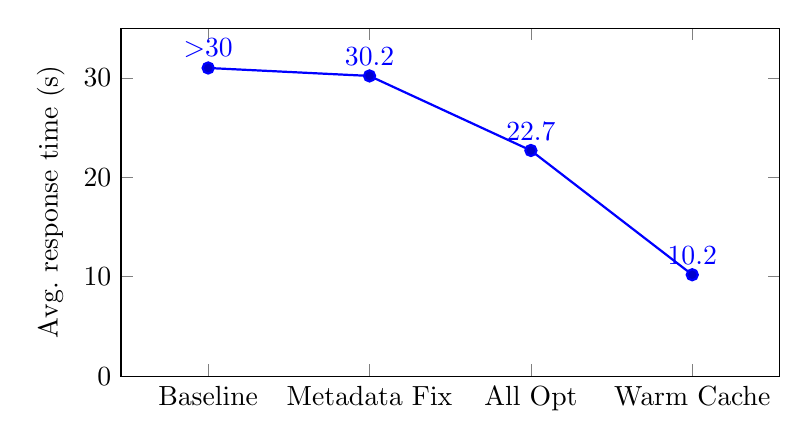
\begin{tikzpicture}
\begin{axis}[symbolic x coords={Baseline,Metadata Fix,All Opt,Warm Cache},
  xtick=data,ymin=0,ymax=35,ylabel={Avg.\ response time (s)},
  width=0.82\textwidth,height=6cm,nodes near coords,point meta=explicit symbolic,
  enlarge x limits=0.18]
\addplot+[mark=*,thick] coordinates
  {(Baseline,31)[$>$30] (Metadata Fix,30.2)[30.2] (All Opt,22.7)[22.7] (Warm Cache,10.2)[10.2]};
\end{axis}
\end{tikzpicture}
\caption{End-to-end RAG latency across optimization phases (average over the
benchmark questions): from over 30\,s to a production-ready $\sim$10.2\,s.}
\label{fig:latency}
\end{figure}

\section{From the First to the Second Iteration}

The first version loaded each record as a single flat document in one mixed-language
collection, retrieved with pure similarity search for all question types, labeled
context chunks numerically, and used a $1024$-token context window. Testing exposed
consistent weaknesses: narrow factual questions returned whole descriptions; structured
queries returned a fixed number of similar documents rather than all matches; English
questions sometimes retrieved Arabic documents; numeric context labels leaked into
answers; some Arabic names were wrong; and short responses were retried with identical
prompts. The second version addressed each as a targeted fix: dataset cleaning,
hierarchical chunking, language-separated collections, the query classifier, removal of
numeric labels, the fifteen-royal Arabic name reference, raised
\texttt{repeat\_penalty} ($1.1\rightarrow1.3$), added \texttt{top\_p} ($0.9$), a larger
context window ($1024\rightarrow4096$), and an augmented-prompt fallback.

\section{API and Deployment}

The pipeline is exposed through a FastAPI server providing \texttt{/ask},
\texttt{/ask/stream} (token streaming), \texttt{/artifact/\{id\}} (structured metadata),
and \texttt{/health}. It runs on a RunPod-hosted NVIDIA RTX A5000 instance (24\,GB
VRAM, 50\,GB RAM, 9 vCPUs) and is reached from the app over an
ngrok tunnel (Figure~\ref{fig:deploy}). At startup the server loads the ChromaDB
collections, reconstructs the indexes, and pre-warms the model so the first visitor
request is already at warm-cache speed.

\begin{figure}[htbp]
\centering
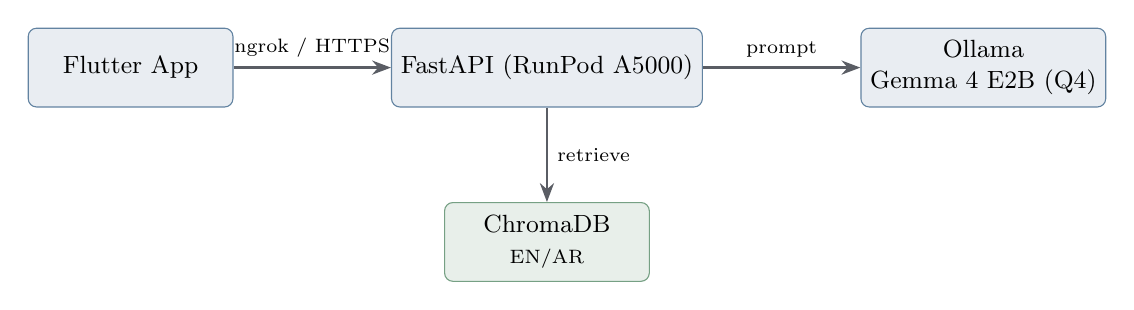
\begin{tikzpicture}[node distance=12mm and 20mm]
  \node[block] (app) {Flutter App};
  \node[block,right=of app] (api) {FastAPI (RunPod A5000)};
  \node[block,right=of api] (gemma) {Ollama\\ Gemma 4 E2B (Q4)};
  \node[store,below=of api] (chroma) {ChromaDB\\\scriptsize EN/AR};
  \draw[flow] (app) -- node[above,font=\scriptsize]{ngrok / HTTPS} (api);
  \draw[flow] (api) -- node[above,font=\scriptsize]{prompt} (gemma);
  \draw[flow] (api) -- node[right,font=\scriptsize]{retrieve} (chroma);
\end{tikzpicture}
\caption{Deployment path: the app reaches the FastAPI RAG service (on a RunPod
RTX A5000 GPU) through an ngrok tunnel; the service retrieves from ChromaDB and
prompts a local Gemma model.}
\label{fig:deploy}
\end{figure}

\section{Results}

On the full evaluation set of thirty questions spanning text mode, camera mode, and
out-of-dataset queries in both Arabic and English, the pipeline averaged about 5.9s
per answer and rated correct on all thirty responses, with no hallucinations, no truncations, 
and no retrieval misses. Performance was uniform across categories: all eight English text-mode questions, 
all six Arabic text-mode questions, all six English camera-mode questions, all three Arabic
camera-mode questions, and all three vague camera-mode questions returned complete, accurate,
well-grounded answers, while all four out-of-dataset queries (Rosetta Stone, Old Kingdom artifacts,
Great Pyramid construction, and the Rosetta Stone in Arabic) were correctly refused
without fabrication. Response times ranged from 4.33s to 8.49s, with Arabic answers
averaging roughly one second slower than English, consistent with Arabic tokenizing to 
about twice the length of equivalent English text. The evaluation also confirmed the pipeline's 
ability to synthesize across separate entries: questions about a single historical figure drew on descriptions
scattered through multiple distinct statue records to assemble a coherent biographical answer rather than
reciting a single chunk. Two cosmetic observations surfaced without affecting correctness  one English 
answer rendered a location name in its raw Arabic form, and another appended a place detail not present
in the source  both minor and isolated against an otherwise clean run.

\section{Limitations}

The knowledge base is closed: questions outside the 108 records receive limited
answers. The query classifier is keyword-based and can misroute a question that avoids
expected vocabulary. The model has no memory across requests, so follow-up questions
are answered without conversational context.

\section{Conclusion}

A fully local, bilingual RAG pipeline---ChromaDB retrieval grounding a quantized
Gemma~4~E2B model behind FastAPI---delivers factual English/Arabic museum answers at
interactive latency. The decisive gains came from grounding and targeted retrieval
fixes, not from a larger model.

\chapter{AR and AI in Museum Tourism: A Market Analysis}

\section{Overview and Scope}

This chapter presents the project's market-research paper: a secondary-research
analysis of intelligent AR guide systems for Egyptian cultural heritage, using the
\GEM{} (GEM) as the case study. It synthesizes academic publications, international
market reports, and tourism statistics to establish the market opportunity, the
competitive landscape, and the user needs that shaped \TimeLens{}. Where it discusses
\TimeLens{} specifically, it refers to the system actually built (on-device YOLOv8n
detection plus a bilingual ChromaDB/Gemma RAG guide), not a broader aspirational
framework.

\section{Market Context}

\subsection{Global AR Trends}
The global Augmented Reality market exceeded USD~50 billion in 2023 and is projected to
surpass USD~110 billion by 2027, supported by more than 1.4
billion smartphone-native AR users and broad ARCore/ARKit availability. The post-COVID
shift toward contactless, mobile-first interaction further accelerated AR adoption in
tourism and cultural heritage~\citep{PwCXR2023}.

\subsection{Egypt's Tourism Market}
Tourism is a primary economic pillar for Egypt, which welcomed approximately 14.9
million international visitors in 2023~\citep{UNWTO2024}, with ancient Egyptian
civilization among the most sought-after global tourism themes. The GEM is expected to
draw between five and eight million visitors annually, and over 70\% of tourists rely
on digital tools during visits~\citep{TGMEgypt2025}, signalling strong demand for
multilingual, mobile-based guidance.

\subsection{Digital Transformation in Museums}
Leading institutions---the Louvre, the British Museum, and the Smithsonian---have
introduced AR-enhanced tours and personalized digital pathways,
and younger audiences engage markedly more with interactive narratives than with static
exhibits~\citep{cho2025augmenting,choiimmersive}. As a flagship international museum, GEM
is expected to adopt comparable digital strategies.

\section{Competitor Landscape and Gap Analysis}

Several tools operate in the museum-technology market, yet none fully meets GEM's
requirements (Table~\ref{tab:competitors}).

\begin{table}[htbp]
\centering
\caption{Competitor landscape for museum guide technology.}
\label{tab:competitors}
\begin{tabularx}{\textwidth}{@{}lXX@{}}
\toprule
\textbf{Solution} & \textbf{Strength} & \textbf{Limitation}\\
\midrule
Google Arts \& Culture & High-quality digital archives, VR tours & No real-time camera recognition; no offline use\\
Smartify & Image recognition for artworks & Requires connectivity; not tuned for Egyptian artifacts\\
British Museum scanning app & Scanning for selected exhibits & No full-gallery coverage\\
Audio guides & Structured information & No interactivity, personalization, or AR\\
QR-code systems & Simple to deploy & Manual scanning interrupts visitor flow\\
\bottomrule
\end{tabularx}
\end{table}

The recurring gaps are: no real-time AI artifact recognition, limited or no offline
functionality, weak Arabic support, a lack of AR overlays and immersive storytelling,
and no GEM-specific experience.

\section{User Needs and Experience}

Secondary research consistently identifies a small set of core needs for AR-enhanced
museum guides: multilingual accessibility, short and digestible
explanations, audio narration~\citep{Ibanez2018}, immediate
real-time recognition~\citep{Radu2014}, and offline operation where connectivity is
unreliable~\citep{Bekele2018}. Behavioral studies show faster AR adoption among
visitors aged 18--35 and a strong preference for mobile guides and personalized
content. The dominant pain points---overwhelming text
labels, difficulty interpreting cultural context, weak connectivity, and time
pressure---map directly onto the design requirements in Chapter~3.

\section{Market Opportunity for a GEM AR Guide}

GEM presents a strong, well-timed opportunity: a vast collection, a large and diverse
international audience, frequently inconsistent in-hall connectivity, and no direct
competitor offering offline, real-time, Arabic-capable artifact recognition. A
dedicated guide that provides instant recognition, short multilingual narration, and
stable offline performance would modernize the visit in line with global standards.

\section{TimeLens Positioning}

\TimeLens{} is designed to fill exactly these gaps with technology that is actually
deployed rather than aspirational:
\begin{itemize}[leftmargin=1.5em]
  \item \textbf{Offline, real-time recognition} via an on-device YOLOv8n detector
        ($5.97$\,MB TFLite), removing the dependence on in-hall connectivity that
        weakens cloud-only competitors. Comparative studies likewise recommend YOLOv8
        for mobile AR recognition~\citep{ipalakova2025comparative}.
  \item \textbf{Bilingual (English/Arabic) grounded narration} via a ChromaDB/Gemma RAG
        guide, addressing the weak-Arabic gap while structurally limiting hallucination.
  \item \textbf{A GEM-specific experience} (51 catalogued artifacts, museum information,
        location gating), which generic platforms do not provide.
\end{itemize}
This positions \TimeLens{} between heavy cloud-AI services and simplistic QR-content
systems: advanced enough to personalize interaction, controlled enough to remain
institutionally trustworthy.

\section{Conclusion and Recommendations}

The market analysis demonstrates a credible product--market fit for an intelligent AR
guide at GEM, driven by global AR growth, Egypt's tourism expansion, visitor digital
behavior, and an unmet need for offline, real-time, Arabic-capable recognition. The
recommended feature set---an offline on-device recognition model, comprehensive
multilingual support, concise audio-visual narration, and clear AR overlays---is the
set \TimeLens{} implements. Remaining steps toward a validated product are primary user
research (including System Usability Scale studies) and a deployment-distribution
evaluation, which are revisited as future work in Chapter~8.

\chapter{Conclusion and Future Work}

\section{Summary of Contributions}

This thesis delivered \TimeLens{}, an AI- and AR-powered bilingual guide for the
\GEM{}, through two engineering contributions and a market study. The first is an
\textbf{on-device artifact detector} whose development isolated label quality---not
architecture or resolution---as the decisive factor, yielding a compact YOLOv8n model
that resolves every previously failing class. The second is a \textbf{grounded
bilingual RAG guide}, selected from a seven-model benchmark and optimized from over
30\,s to about 10\,s end-to-end latency, that keeps answers anchored to curated museum
data in English or Arabic. Both ship in a production Flutter application, and a market
analysis situates the system within the heritage-AR landscape.

\section{Critical Reflection}

The decisive gains in this project came not from model complexity but from
\textbf{clean data and grounding}: hand-verified labels made the on-device detector
trustworthy, and retrieval grounding kept the language model factual. The honest
residual risks are equally clear---validation frame leakage and training-to-deployment
domain shift on the detection side, fine-grained long-tail classes, and evolving
real-world capture conditions.

\section{Future Work}

\paragraph{Detection.} Split the dataset by source video rather than by frame to remove
frame leakage; capture and annotate a phone-camera \emph{deployment-distribution} test
set for honest field metrics; apply stronger augmentation for domain shift; and
re-label or expand the remaining long-tail classes.

\paragraph{Retrieval-augmented guide.} Expand the closed knowledge base; replace or
augment the keyword query classifier with a learned intent model; add conversational
memory across turns; and build index health-audit and maintenance tooling so the
knowledge base can be updated and validated routinely as the collection grows.

\paragraph{System.} Optionally enable backend re-verification (the \texttt{/predict}
path) for low-confidence detections; add explainable detection overlays; and conduct
primary user studies (including System Usability Scale evaluation) in live museum
conditions to quantify learning outcomes and long-horizon experience quality.


% ---------------------------------------------------------------- back
\appendix
\chapter{AI Ethics and Bias Statement}

\section{Data Fairness}
We assess class balance and confusion concentration to detect under-represented
categories and biased behavior. Per-class precision/recall/mAP (recorded in the
detector's \texttt{per\_class\_metrics.csv}) and the normalized confusion matrix expose
the fine-grained classes most prone to error, rather than hiding them behind an average.

\section{Mitigation}
Bias and failure are mitigated primarily through \emph{label quality}: hand annotation
removed systematic auto-labeling errors, augmentation broadens coverage, and per-class
confidence thresholds (e.g., a stricter floor for the false-positive-prone
\emph{Siptah Stela}) reduce confident mistakes. On the language side, retrieval
grounding plus an explicit Arabic name reference reduce hallucination and mis-transliteration.

\section{Transparency and Explainability}
The work reports per-class metrics and the confusion matrix, and openly discloses the
validation frame-leakage and domain-shift limitations together with conservative
held-out numbers. The RAG guide answers only from retrieved, citable museum context.

\section{Ethical Risk Assessment}
The principal risk is misplaced visitor trust in an uncertain prediction. The system
mitigates this with a calibrated confidence gate that suppresses low-confidence
detections rather than guessing, on-device inference that uploads no per-frame imagery,
and a locally served language model that keeps visitor queries out of third-party
services.

\chapter{Reproducibility Report}

\section{Environment}
The detector is trained with Ultralytics 8.4.45 on PyTorch; the RAG service uses
FastAPI, LlamaIndex, LangChain, Ollama, and ChromaDB; the mobile app is built with
Flutter. Dependency definitions and scripts in the project repositories support
deterministic re-runs.

\section{Deployment}
The RAG service is deployed on a RunPod RTX A5000 instance and exposed to the mobile
app through an
ngrok tunnel; the detector ships as a TensorFlow Lite asset bundled with the Flutter
app. No container image is required for the deployed path.

\section{Seed and Split Management}
Because the dataset is built from video frames, splits are performed
\emph{chronologically within each class/video group} (not by random shuffle) to
minimize near-duplicate frame leakage between train, validation, and test. The v3
detector uses a $70/20/10$ split.

\section{Hardware}
Table~\ref{tab:hardware} reports the hardware used for each role.

\begin{table}[htbp]
\centering
\caption{Hardware and runtime by role.}
\label{tab:hardware}
\begin{tabularx}{\textwidth}{@{}l>{\raggedright\arraybackslash}p{0.30\textwidth}>{\raggedright\arraybackslash}X@{}}
\toprule
\textbf{Role} & \textbf{Hardware} & \textbf{Notes}\\
\midrule
Detector training & NVIDIA GTX 1650 Ti (4\,GB) & Ultralytics 8.4.45 / PyTorch; $\sim$34\,h GPU $+$ $\sim$40\,h hand annotation.\\
RAG experiments   & NVIDIA RTX 3050 Laptop (4\,GB), 16\,GB RAM & Ollama (CUDA), Flash Attention enabled.\\
Production serving & RunPod NVIDIA RTX A5000 (24\,GB VRAM) $+$ ngrok & FastAPI RAG
service; 9 vCPU (Intel Xeon Gold 6342 @ 2.80\,GHz), 50\,GB RAM, 30\,GB storage.\\
\bottomrule
\end{tabularx}
\end{table}

\section{Experiment Traceability}
Detector experiments are traceable through the Ultralytics run directories
(\texttt{results.csv}, \texttt{per\_class\_metrics.csv}) for each iteration
(v1/v2/v2@640/v3). The RAG pipeline is evaluated against a fixed set of 20 standardized
bilingual questions (12 English, 8 Arabic) across camera and text modes.

\section{One-Command Rebuild}
The detector is reproduced by running the training scripts
\texttt{01\allowbreak\_split\allowbreak\_dataset.py} through \texttt{06\_eval.py} and exporting
with \texttt{05\_export\allowbreak\_tflite.py}; the knowledge service is rebuilt with
\texttt{index\_dataset.py} and served with \texttt{api.py}.

\chapter{Generative AI Disclosure}

\section{Tool Inventory}
Generative-AI assistance (GitHub Copilot and related large-language-model tools) was
used for drafting support, boilerplate acceleration, and editing suggestions across the
code and this document.

\section{Usage Scope}
GenAI was used for drafting and revision support. Core design choices, the experimental
protocol, the data-quality iteration, model selection, and all reported results remained
human-led.

\section{Verification Statement}
All AI-assisted text and code suggestions were manually reviewed, corrected where
necessary, and validated against repository evidence (training runs, evaluation
artifacts, and the RAG benchmark) before acceptance.

\section{Critical Audit Log}
At least one audit cycle is recorded in which a generated suggestion was inaccurate and
corrected before inclusion: an early draft described the detector as ``YOLOv11'' and the
vector store as ``FAISS''; both were corrected to the actual YOLOv8n detector and
ChromaDB store after verification against the training and RAG repositories.


\cleardoublepage
\bibliographystyle{IEEEtran}   % fallback: plainnat
\bibliography{references}

% =====================================================================
%  Arabic-language abstract (الملخّص).
%  Typeset with native Arabic (polyglossia + Amiri), set up in preamble.tex.
%  REQUIRES a Unicode engine (XeLaTeX/LuaLaTeX). Under pdfLaTeX it degrades
%  to a one-line notice so the document still compiles.
%  Latin technical tokens are wrapped in \textenglish{...} so they render
%  left-to-right in Latin Modern; numerals=maghrib keeps digits Western.
% =====================================================================

\ifPDFTeX
\chapter*{Abstract (Arabic)}
\addcontentsline{toc}{chapter}{Abstract (Arabic)}
\noindent\textit{The Arabic-language abstract is typeset with native Arabic and
requires compilation with XeLaTeX or LuaLaTeX (\texttt{latexmk main.tex}).}
\else
\begin{otherlanguage}{arabic}
\chapter*{المستخلص}
\addcontentsline{toc}{chapter}{\textenglish{Abstract (Arabic)}}

توثّق هذه الرسالة تصميم نظام تايم لنز (\textenglish{\TimeLens{}}) وتنفيذه وتقييمه، وهو دليلٌ
إرشاديٌّ للأجهزة المحمولة مدعومٌ بالذكاء الاصطناعي والواقع المعزَّز، ومخصَّصٌ
للمتحف المصري الكبير (\textenglish{GEM}). فبمجرّد توجيه الهاتف نحو إحدى القطع
المعروضة، يرى الزائرُ القطعةَ الأثرية وقد جرى التعرّف عليها في الزمن الحقيقي،
ويمكنه طرح أسئلة متابعة تُجاب بالعربية أو الإنجليزية. ويتصدّى هذا العمل لثلاث
مشكلات ترتبط تحديدًا بالتشغيل داخل قاعات العرض: التشابه البصري الدقيق بين
\textenglish{51} قطعة أثرية مُفهرَسة (كثيرٌ منها تماثيل رمسيسية شبه متطابقة)، والفجوة بين بيانات
التدريب المنسَّقة وظروف التصوير بكاميرا الهاتف المحمول، وخطر أن يذكر الدليلُ
الذكيُّ «حقائق» تاريخية لا يستطيع إسنادها.

تُقدّم الرسالة إسهامَين بحثيَّين هندسيَّين ودراسةً سوقية. الإسهام الأول كاشفٌ
للقطع الأثرية يعمل على الجهاز نفسه، طُوِّر عبر دراسة تَكرارية موجَّهة بجودة
البيانات: بدءًا من التوسيم الآلي بنموذج أساس (\textenglish{YOLO-World})، مرورًا
بقواعد مكانية لتنقية التوسيمات، وصولًا إلى مجموعة بيانات موسومة يدويًا بالكامل.
وتَعزِل الدراسةُ جودةَ التوسيم — لا معماريةَ النموذج ولا دقةَ الدخل — بوصفها
العاملَ الحاسم: إذ يَحُلّ نموذج \textenglish{YOLOv8n} النهائي كلَّ فئة كانت تفشل
سابقًا، مع بقائه أصلًا بصيغة \textenglish{TensorFlow Lite} لا يتجاوز حجمه
\textenglish{5.97} ميغابايت ويعمل في الزمن الحقيقي على هاتف متوسط الإمكانات. أمّا الإسهام
الثاني فهو دليلٌ ثنائي اللغة قائمٌ على التوليد المعزَّز بالاسترجاع
(\textenglish{RAG}) ومُسنَدٌ إلى قاعدة معرفة من 108 سجلات في \textenglish{ChromaDB}؛
وقد اختار تقييمٌ منهجيٌّ لسبعة نماذج لغوية مرشَّحة النموذجَ
\textenglish{Gemma 4 E2B (Q4\_K\_M)}، كما خفّض تحسينٌ من عشر خطوات زمنَ الاستجابة
الكلي من أكثر من \textenglish{30} ثانية إلى نحو \textenglish{10} ثوانٍ. ويُدمَج الإسهامان معًا في تطبيق
\textenglish{Flutter} جاهزٍ للإنتاج، مع واجهة ثنائية اللغة، وتقييدٍ حسب موقع
المتحف، وخاصيةِ تحويل النص إلى كلام.

% وإلى جانب النتائج الرئيسية، كُتبت الرسالة لتكون قابلةً لإعادة الإنتاج وصادقةً
% بشأن حدودها: إذ تُفصِح دراسة الكشف صراحةً عن تسرّب الإطارات في بيانات التحقّق
% وعن انزياح المجال بين بيئة التدريب وبيئة التشغيل، وتُورِد نتيجة متحفِّظة على
% بيانات محجوزة (\textenglish{mAP@0.5 = 0.751}) إلى جانب نتائج البيانات داخل
% التوزيع. ويتضمّن المستند ملاحظاتٍ لإعادة الإنتاج، وبيانًا للأخلاقيات والتحيُّز،
% وإفصاحًا رسميًا عن استخدام الذكاء الاصطناعي التوليدي.

وإلى جانب المقاييس الرئيسية، تُورِد الرسالة نتيجةً متحفِّظة على بيانات
محجوزة (\textenglish{mAP@0.5 = 0.751}) إلى جانب نتائج البيانات داخل
التوزيع. ويتضمّن المستند ملاحظاتٍ لإعادة الإنتاج، وبيانًا للأخلاقيات
والتحيُّز، وإفصاحًا رسميًا عن استخدام الذكاء الاصطناعي التوليدي.

\vspace{1.2em}
\noindent\textbf{الكلمات المفتاحية:} كشف الأجسام على الجهاز؛ \textenglish{YOLOv8n}؛
\textenglish{TensorFlow Lite}؛ التوليد المعزَّز بالاسترجاع (\textenglish{RAG})؛
\textenglish{Gemma}؛ \textenglish{ChromaDB}؛ الإجابة عن الأسئلة ثنائية اللغة؛
الواقع المعزَّز؛ \textenglish{Flutter}؛ حوسبة التراث الثقافي؛ المتحف المصري الكبير.
\end{otherlanguage}
\fi

\begin{titlepage}
\thispagestyle{empty}
\centering

\begin{center}
\includegraphics[width=0.18\linewidth]{uni\_logo.png}
\end{center}
\begin{otherlanguage}{arabic}
{\small جامعة العاصمة (جـامـعـة حـلـوان سابقاً)\par}
{\small كـليـة الحـاسـبـات والـذكـاء الاصطناعي\par}
{\small قـسـم الذكاء الاصطناعي\par}

\vspace{8mm}
{\Large\bfseries تايم لنز:\\
تطبيق للتعرُّف علي القطع الأثرية\\
وإجابة الأسئلة مُعزَّز بالاسترجاع\\
 للمتحف المصري الكبير
\par}
\vspace{8mm}

رسالة مشروع تخرج مقدمة من:\\
\vfill
\begin{tabular}{@{}ll@{}}
	{\large روان هشام \par} & {\large \textenglish{[20220167]}\par}\\
	{\large علي أشرف  \par} & {\large \textenglish{[20220296]}\par}\\
	{\large عمر أحمد  \par} & {\large \textenglish{[20220310]}\par}\\
	{\large عمر وجيه  \par} & {\large \textenglish{[20220324]}\par}\\
	{\large عمرو أحمد \par} & {\large \textenglish{[20210632]}\par}\\
	{\large ملك علاء   \par} & {\large \textenglish{[20220503]}\par}\\
\end{tabular}
\vfill
رسالة مقدمة ضمن متطلبات الحصول على درجة البكالوريوس في الحاسبات والذكاء الاصطناعي، بقسم الذكاء الاصطناعي، كلية الحاسبات والذكاء الاصطناعي، جامعة العاصمة (جامعة حلوان سابقاً)\\
\vfill
تحت إشراف:\\
{\large د. إسلام جمال\par}
\vfill
يونيو \textenglish{2026}
\end{otherlanguage}
\end{titlepage}

\end{document}

